% Options for packages loaded elsewhere
\PassOptionsToPackage{unicode}{hyperref}
\PassOptionsToPackage{hyphens}{url}
\PassOptionsToPackage{dvipsnames,svgnames,x11names}{xcolor}
%
\documentclass[
  letterpaper,
  DIV=11,
  numbers=noendperiod]{scrartcl}

\usepackage{amsmath,amssymb}
\usepackage{iftex}
\ifPDFTeX
  \usepackage[T1]{fontenc}
  \usepackage[utf8]{inputenc}
  \usepackage{textcomp} % provide euro and other symbols
\else % if luatex or xetex
  \usepackage{unicode-math}
  \defaultfontfeatures{Scale=MatchLowercase}
  \defaultfontfeatures[\rmfamily]{Ligatures=TeX,Scale=1}
\fi
\usepackage{lmodern}
\ifPDFTeX\else  
    % xetex/luatex font selection
\fi
% Use upquote if available, for straight quotes in verbatim environments
\IfFileExists{upquote.sty}{\usepackage{upquote}}{}
\IfFileExists{microtype.sty}{% use microtype if available
  \usepackage[]{microtype}
  \UseMicrotypeSet[protrusion]{basicmath} % disable protrusion for tt fonts
}{}
\makeatletter
\@ifundefined{KOMAClassName}{% if non-KOMA class
  \IfFileExists{parskip.sty}{%
    \usepackage{parskip}
  }{% else
    \setlength{\parindent}{0pt}
    \setlength{\parskip}{6pt plus 2pt minus 1pt}}
}{% if KOMA class
  \KOMAoptions{parskip=half}}
\makeatother
\usepackage{xcolor}
\setlength{\emergencystretch}{3em} % prevent overfull lines
\setcounter{secnumdepth}{-\maxdimen} % remove section numbering
% Make \paragraph and \subparagraph free-standing
\makeatletter
\ifx\paragraph\undefined\else
  \let\oldparagraph\paragraph
  \renewcommand{\paragraph}{
    \@ifstar
      \xxxParagraphStar
      \xxxParagraphNoStar
  }
  \newcommand{\xxxParagraphStar}[1]{\oldparagraph*{#1}\mbox{}}
  \newcommand{\xxxParagraphNoStar}[1]{\oldparagraph{#1}\mbox{}}
\fi
\ifx\subparagraph\undefined\else
  \let\oldsubparagraph\subparagraph
  \renewcommand{\subparagraph}{
    \@ifstar
      \xxxSubParagraphStar
      \xxxSubParagraphNoStar
  }
  \newcommand{\xxxSubParagraphStar}[1]{\oldsubparagraph*{#1}\mbox{}}
  \newcommand{\xxxSubParagraphNoStar}[1]{\oldsubparagraph{#1}\mbox{}}
\fi
\makeatother

\usepackage{color}
\usepackage{fancyvrb}
\newcommand{\VerbBar}{|}
\newcommand{\VERB}{\Verb[commandchars=\\\{\}]}
\DefineVerbatimEnvironment{Highlighting}{Verbatim}{commandchars=\\\{\}}
% Add ',fontsize=\small' for more characters per line
\usepackage{framed}
\definecolor{shadecolor}{RGB}{241,243,245}
\newenvironment{Shaded}{\begin{snugshade}}{\end{snugshade}}
\newcommand{\AlertTok}[1]{\textcolor[rgb]{0.68,0.00,0.00}{#1}}
\newcommand{\AnnotationTok}[1]{\textcolor[rgb]{0.37,0.37,0.37}{#1}}
\newcommand{\AttributeTok}[1]{\textcolor[rgb]{0.40,0.45,0.13}{#1}}
\newcommand{\BaseNTok}[1]{\textcolor[rgb]{0.68,0.00,0.00}{#1}}
\newcommand{\BuiltInTok}[1]{\textcolor[rgb]{0.00,0.23,0.31}{#1}}
\newcommand{\CharTok}[1]{\textcolor[rgb]{0.13,0.47,0.30}{#1}}
\newcommand{\CommentTok}[1]{\textcolor[rgb]{0.37,0.37,0.37}{#1}}
\newcommand{\CommentVarTok}[1]{\textcolor[rgb]{0.37,0.37,0.37}{\textit{#1}}}
\newcommand{\ConstantTok}[1]{\textcolor[rgb]{0.56,0.35,0.01}{#1}}
\newcommand{\ControlFlowTok}[1]{\textcolor[rgb]{0.00,0.23,0.31}{\textbf{#1}}}
\newcommand{\DataTypeTok}[1]{\textcolor[rgb]{0.68,0.00,0.00}{#1}}
\newcommand{\DecValTok}[1]{\textcolor[rgb]{0.68,0.00,0.00}{#1}}
\newcommand{\DocumentationTok}[1]{\textcolor[rgb]{0.37,0.37,0.37}{\textit{#1}}}
\newcommand{\ErrorTok}[1]{\textcolor[rgb]{0.68,0.00,0.00}{#1}}
\newcommand{\ExtensionTok}[1]{\textcolor[rgb]{0.00,0.23,0.31}{#1}}
\newcommand{\FloatTok}[1]{\textcolor[rgb]{0.68,0.00,0.00}{#1}}
\newcommand{\FunctionTok}[1]{\textcolor[rgb]{0.28,0.35,0.67}{#1}}
\newcommand{\ImportTok}[1]{\textcolor[rgb]{0.00,0.46,0.62}{#1}}
\newcommand{\InformationTok}[1]{\textcolor[rgb]{0.37,0.37,0.37}{#1}}
\newcommand{\KeywordTok}[1]{\textcolor[rgb]{0.00,0.23,0.31}{\textbf{#1}}}
\newcommand{\NormalTok}[1]{\textcolor[rgb]{0.00,0.23,0.31}{#1}}
\newcommand{\OperatorTok}[1]{\textcolor[rgb]{0.37,0.37,0.37}{#1}}
\newcommand{\OtherTok}[1]{\textcolor[rgb]{0.00,0.23,0.31}{#1}}
\newcommand{\PreprocessorTok}[1]{\textcolor[rgb]{0.68,0.00,0.00}{#1}}
\newcommand{\RegionMarkerTok}[1]{\textcolor[rgb]{0.00,0.23,0.31}{#1}}
\newcommand{\SpecialCharTok}[1]{\textcolor[rgb]{0.37,0.37,0.37}{#1}}
\newcommand{\SpecialStringTok}[1]{\textcolor[rgb]{0.13,0.47,0.30}{#1}}
\newcommand{\StringTok}[1]{\textcolor[rgb]{0.13,0.47,0.30}{#1}}
\newcommand{\VariableTok}[1]{\textcolor[rgb]{0.07,0.07,0.07}{#1}}
\newcommand{\VerbatimStringTok}[1]{\textcolor[rgb]{0.13,0.47,0.30}{#1}}
\newcommand{\WarningTok}[1]{\textcolor[rgb]{0.37,0.37,0.37}{\textit{#1}}}

\providecommand{\tightlist}{%
  \setlength{\itemsep}{0pt}\setlength{\parskip}{0pt}}\usepackage{longtable,booktabs,array}
\usepackage{calc} % for calculating minipage widths
% Correct order of tables after \paragraph or \subparagraph
\usepackage{etoolbox}
\makeatletter
\patchcmd\longtable{\par}{\if@noskipsec\mbox{}\fi\par}{}{}
\makeatother
% Allow footnotes in longtable head/foot
\IfFileExists{footnotehyper.sty}{\usepackage{footnotehyper}}{\usepackage{footnote}}
\makesavenoteenv{longtable}
\usepackage{graphicx}
\makeatletter
\def\maxwidth{\ifdim\Gin@nat@width>\linewidth\linewidth\else\Gin@nat@width\fi}
\def\maxheight{\ifdim\Gin@nat@height>\textheight\textheight\else\Gin@nat@height\fi}
\makeatother
% Scale images if necessary, so that they will not overflow the page
% margins by default, and it is still possible to overwrite the defaults
% using explicit options in \includegraphics[width, height, ...]{}
\setkeys{Gin}{width=\maxwidth,height=\maxheight,keepaspectratio}
% Set default figure placement to htbp
\makeatletter
\def\fps@figure{htbp}
\makeatother

\usepackage{fvextra}
\DefineVerbatimEnvironment{Highlighting}{Verbatim}{breaklines,commandchars=\\\{\}}
\KOMAoption{captions}{tableheading}
\makeatletter
\@ifpackageloaded{caption}{}{\usepackage{caption}}
\AtBeginDocument{%
\ifdefined\contentsname
  \renewcommand*\contentsname{Table of contents}
\else
  \newcommand\contentsname{Table of contents}
\fi
\ifdefined\listfigurename
  \renewcommand*\listfigurename{List of Figures}
\else
  \newcommand\listfigurename{List of Figures}
\fi
\ifdefined\listtablename
  \renewcommand*\listtablename{List of Tables}
\else
  \newcommand\listtablename{List of Tables}
\fi
\ifdefined\figurename
  \renewcommand*\figurename{Figure}
\else
  \newcommand\figurename{Figure}
\fi
\ifdefined\tablename
  \renewcommand*\tablename{Table}
\else
  \newcommand\tablename{Table}
\fi
}
\@ifpackageloaded{float}{}{\usepackage{float}}
\floatstyle{ruled}
\@ifundefined{c@chapter}{\newfloat{codelisting}{h}{lop}}{\newfloat{codelisting}{h}{lop}[chapter]}
\floatname{codelisting}{Listing}
\newcommand*\listoflistings{\listof{codelisting}{List of Listings}}
\makeatother
\makeatletter
\makeatother
\makeatletter
\@ifpackageloaded{caption}{}{\usepackage{caption}}
\@ifpackageloaded{subcaption}{}{\usepackage{subcaption}}
\makeatother

\ifLuaTeX
  \usepackage{selnolig}  % disable illegal ligatures
\fi
\usepackage{bookmark}

\IfFileExists{xurl.sty}{\usepackage{xurl}}{} % add URL line breaks if available
\urlstyle{same} % disable monospaced font for URLs
\hypersetup{
  pdftitle={Final Project: Code},
  pdfauthor={Duoshu Xu \& Jae Hu \& Regina Hou},
  colorlinks=true,
  linkcolor={blue},
  filecolor={Maroon},
  citecolor={Blue},
  urlcolor={Blue},
  pdfcreator={LaTeX via pandoc}}


\title{Final Project: Code}
\author{Duoshu Xu \& Jae Hu \& Regina Hou}
\date{}

\begin{document}
\maketitle

\RecustomVerbatimEnvironment{verbatim}{Verbatim}{
  showspaces = false,
  showtabs = false,
  breaksymbolleft={},
  breaklines
}


\begin{Shaded}
\begin{Highlighting}[]
\ImportTok{import}\NormalTok{ pandas }\ImportTok{as}\NormalTok{ pd}
\ImportTok{import}\NormalTok{ numpy }\ImportTok{as}\NormalTok{ np}
\ImportTok{import}\NormalTok{ altair }\ImportTok{as}\NormalTok{ alt}
\ImportTok{import}\NormalTok{ pandas }\ImportTok{as}\NormalTok{ pd}
\ImportTok{import}\NormalTok{ matplotlib.pyplot }\ImportTok{as}\NormalTok{ plt}
\end{Highlighting}
\end{Shaded}

\begin{Shaded}
\begin{Highlighting}[]
\NormalTok{file\_path }\OperatorTok{=} \StringTok{\textquotesingle{}/Users/kevinxu/Desktop/Final Project Raw Data/mapdataall.csv\textquotesingle{}}
\NormalTok{wildfire\_data }\OperatorTok{=}\NormalTok{ pd.read\_csv(file\_path)}
\end{Highlighting}
\end{Shaded}

\begin{Shaded}
\begin{Highlighting}[]
\NormalTok{file\_path }\OperatorTok{=} \StringTok{\textquotesingle{}/Users/kevinxu/Desktop/Final Project Data Cleaning/Census data.xlsx\textquotesingle{}}
\NormalTok{census\_data }\OperatorTok{=}\NormalTok{ pd.read\_excel(file\_path)}
\end{Highlighting}
\end{Shaded}

\section{Data cleaning and reshaping (done by Jae
Hu)}\label{data-cleaning-and-reshaping-done-by-jae-hu}

\begin{Shaded}
\begin{Highlighting}[]
\NormalTok{census\_data[}\StringTok{\textquotesingle{}Total Population\textquotesingle{}}\NormalTok{] }\OperatorTok{=}\NormalTok{ pd.to\_numeric(}
\NormalTok{    census\_data[}\StringTok{\textquotesingle{}Total Population\textquotesingle{}}\NormalTok{], errors}\OperatorTok{=}\StringTok{\textquotesingle{}coerce\textquotesingle{}}\NormalTok{)}


\KeywordTok{def}\NormalTok{ classify\_geographic\_type(population):}
    \ControlFlowTok{if}\NormalTok{ population }\OperatorTok{\textgreater{}} \DecValTok{50000}\NormalTok{:}
        \ControlFlowTok{return} \StringTok{"Urban"}
    \ControlFlowTok{elif} \DecValTok{5000} \OperatorTok{\textless{}=}\NormalTok{ population }\OperatorTok{\textless{}=} \DecValTok{50000}\NormalTok{:}
        \ControlFlowTok{return} \StringTok{"Suburban"}
    \ControlFlowTok{else}\NormalTok{:}
        \ControlFlowTok{return} \StringTok{"Rural"}


\NormalTok{census\_data[}\StringTok{\textquotesingle{}geographic type\textquotesingle{}}\NormalTok{] }\OperatorTok{=}\NormalTok{ census\_data[}\StringTok{\textquotesingle{}Total Population\textquotesingle{}}\NormalTok{].}\BuiltInTok{apply}\NormalTok{(}
\NormalTok{    classify\_geographic\_type)}

\NormalTok{output\_file\_path }\OperatorTok{=} \StringTok{\textquotesingle{}/Users/kevinxu/Desktop/Final Project Raw Data/Census\_with\_types.csv\textquotesingle{}}

\NormalTok{census\_data.to\_csv(output\_file\_path, index}\OperatorTok{=}\VariableTok{False}\NormalTok{)}
\end{Highlighting}
\end{Shaded}

\section{pie chart (done by Jae Hu)}\label{pie-chart-done-by-jae-hu}

\begin{Shaded}
\begin{Highlighting}[]
\CommentTok{\# Load the modified Census data}
\NormalTok{file\_path }\OperatorTok{=} \StringTok{\textquotesingle{}/Users/kevinxu/Desktop/Final Project Raw Data/Census\_with\_types.csv\textquotesingle{}}
\NormalTok{census\_data }\OperatorTok{=}\NormalTok{ pd.read\_csv(file\_path)}

\CommentTok{\# Count the number of cities in each geographic type}
\NormalTok{geo\_counts }\OperatorTok{=}\NormalTok{ census\_data[}\StringTok{\textquotesingle{}geographic type\textquotesingle{}}\NormalTok{].value\_counts()}

\CommentTok{\# Define a custom autopct function to add both percentages and counts}
\KeywordTok{def}\NormalTok{ autopct\_with\_counts(pct):}
\NormalTok{    count }\OperatorTok{=} \BuiltInTok{int}\NormalTok{(}\BuiltInTok{round}\NormalTok{(pct }\OperatorTok{*}\NormalTok{ geo\_counts.}\BuiltInTok{sum}\NormalTok{() }\OperatorTok{/} \FloatTok{100.0}\NormalTok{))}
    \ControlFlowTok{return} \SpecialStringTok{f\textquotesingle{}}\SpecialCharTok{\{}\NormalTok{pct}\SpecialCharTok{:.1f\}}\SpecialStringTok{\%}\CharTok{\textbackslash{}n}\SpecialStringTok{(}\SpecialCharTok{\{}\NormalTok{count}\SpecialCharTok{\}}\SpecialStringTok{)\textquotesingle{}}  

\CommentTok{\# Plot the pie chart}
\NormalTok{plt.figure(figsize}\OperatorTok{=}\NormalTok{(}\DecValTok{8}\NormalTok{, }\DecValTok{8}\NormalTok{))}
\NormalTok{colors }\OperatorTok{=}\NormalTok{ [}\StringTok{"lightcyan"}\NormalTok{, }\StringTok{"powderblue"}\NormalTok{, }\StringTok{"cadetblue"}\NormalTok{]  }
\NormalTok{geo\_counts.plot.pie(}
\NormalTok{    autopct}\OperatorTok{=}\NormalTok{autopct\_with\_counts,  }
\NormalTok{    colors}\OperatorTok{=}\NormalTok{colors,}
\NormalTok{    startangle}\OperatorTok{=}\DecValTok{90}\NormalTok{,}
\NormalTok{    labels}\OperatorTok{=}\NormalTok{geo\_counts.index,  }
\NormalTok{    wedgeprops}\OperatorTok{=}\NormalTok{\{}\StringTok{"edgecolor"}\NormalTok{: }\StringTok{"black"}\NormalTok{\} }
\NormalTok{)}

\CommentTok{\# Add title}
\NormalTok{plt.title(}\StringTok{"Distribution of Rural, Suburban, and Urban Cities in California"}\NormalTok{, fontsize}\OperatorTok{=}\DecValTok{14}\NormalTok{)}

\CommentTok{\# Show the chart}
\NormalTok{plt.ylabel(}\StringTok{""}\NormalTok{) }
\NormalTok{plt.show()}
\end{Highlighting}
\end{Shaded}

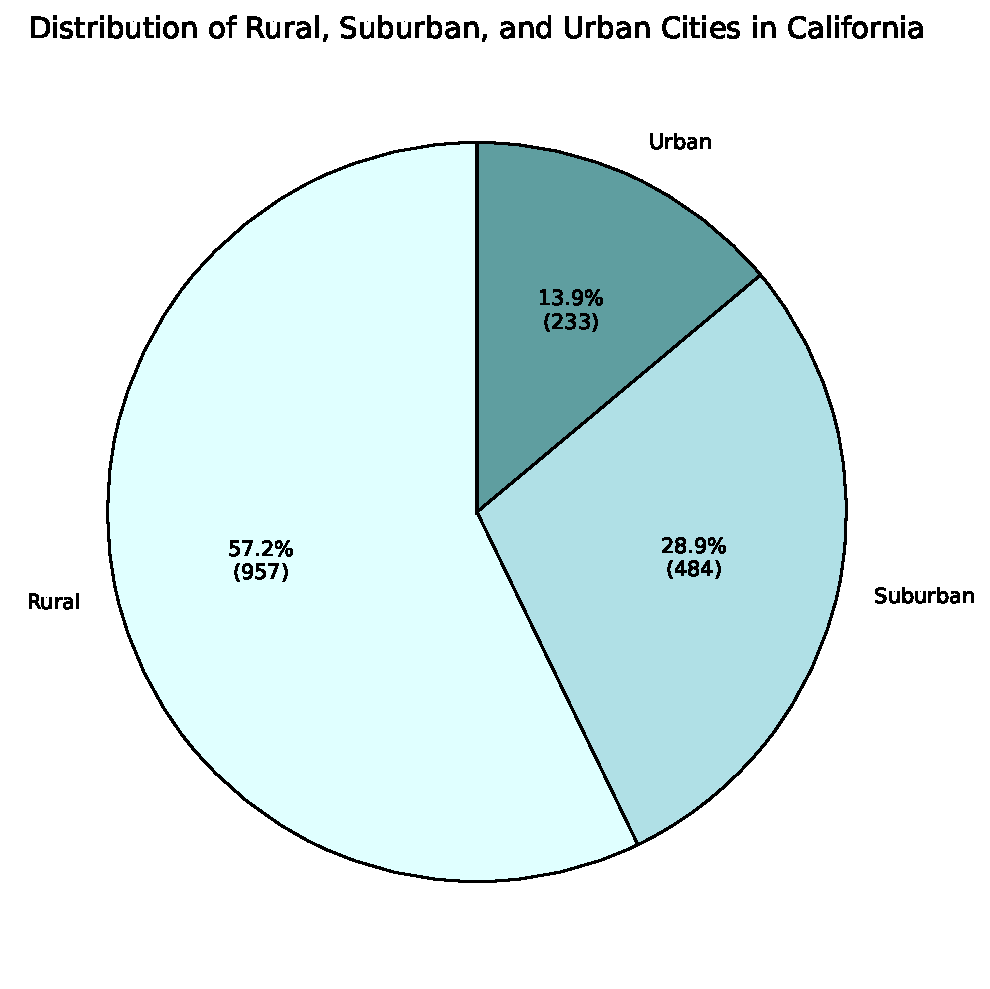
\includegraphics{Final Code_files/figure-pdf/cell-6-output-1.pdf}

\section{Wildfire Frequency bar chart (done by Duoshu
Xu)}\label{wildfire-frequency-bar-chart-done-by-duoshu-xu}

\begin{Shaded}
\begin{Highlighting}[]
\NormalTok{wildfire\_data\_path }\OperatorTok{=} \StringTok{\textquotesingle{}/Users/kevinxu/Desktop/Final Project Raw Data/mapdataall.csv\textquotesingle{}}
\NormalTok{census\_data\_path }\OperatorTok{=} \StringTok{\textquotesingle{}/Users/kevinxu/Desktop/Final Project Raw Data/Census\_with\_types.csv\textquotesingle{}}
\NormalTok{wildfire\_data }\OperatorTok{=}\NormalTok{ pd.read\_csv(wildfire\_data\_path)}
\NormalTok{census\_data }\OperatorTok{=}\NormalTok{ pd.read\_csv(census\_data\_path)}


\KeywordTok{def}\NormalTok{ standardize\_county\_name(name):}
    \ControlFlowTok{if}\NormalTok{ pd.isna(name):}
        \ControlFlowTok{return} \VariableTok{None}
    \ControlFlowTok{return}\NormalTok{ name.split(}\StringTok{","}\NormalTok{)[}\DecValTok{0}\NormalTok{].strip()}


\NormalTok{wildfire\_data[}\StringTok{\textquotesingle{}incident\_county\_cleaned\textquotesingle{}}\NormalTok{] }\OperatorTok{=}\NormalTok{ wildfire\_data[}\StringTok{\textquotesingle{}incident\_county\textquotesingle{}}\NormalTok{].}\BuiltInTok{apply}\NormalTok{(}
\NormalTok{    standardize\_county\_name)}
\NormalTok{census\_data[}\StringTok{\textquotesingle{}Geography\_cleaned\textquotesingle{}}\NormalTok{] }\OperatorTok{=}\NormalTok{ census\_data[}\StringTok{\textquotesingle{}Geography\textquotesingle{}}\NormalTok{].}\BuiltInTok{str}\NormalTok{.replace(}
    \StringTok{" County"}\NormalTok{, }\StringTok{""}\NormalTok{, regex}\OperatorTok{=}\VariableTok{False}\NormalTok{)}

\NormalTok{wildfire\_with\_geo\_type }\OperatorTok{=}\NormalTok{ wildfire\_data.merge(}
\NormalTok{    census\_data[[}\StringTok{\textquotesingle{}Geography\_cleaned\textquotesingle{}}\NormalTok{, }\StringTok{\textquotesingle{}geographic type\textquotesingle{}}\NormalTok{]],}
\NormalTok{    left\_on}\OperatorTok{=}\StringTok{\textquotesingle{}incident\_county\_cleaned\textquotesingle{}}\NormalTok{,}
\NormalTok{    right\_on}\OperatorTok{=}\StringTok{\textquotesingle{}Geography\_cleaned\textquotesingle{}}\NormalTok{,}
\NormalTok{    how}\OperatorTok{=}\StringTok{\textquotesingle{}left\textquotesingle{}}
\NormalTok{)}

\NormalTok{wildfire\_counts }\OperatorTok{=}\NormalTok{ wildfire\_with\_geo\_type[}\StringTok{\textquotesingle{}geographic type\textquotesingle{}}\NormalTok{].value\_counts(}
\NormalTok{).reset\_index()}
\NormalTok{wildfire\_counts.columns }\OperatorTok{=}\NormalTok{ [}\StringTok{\textquotesingle{}Geographic Type\textquotesingle{}}\NormalTok{, }\StringTok{\textquotesingle{}Number of Wildfires\textquotesingle{}}\NormalTok{]}

\BuiltInTok{print}\NormalTok{(wildfire\_counts)}
\NormalTok{plt.figure(figsize}\OperatorTok{=}\NormalTok{(}\DecValTok{10}\NormalTok{, }\DecValTok{6}\NormalTok{))}
\NormalTok{plt.bar(}
\NormalTok{    wildfire\_counts[}\StringTok{\textquotesingle{}Geographic Type\textquotesingle{}}\NormalTok{],}
\NormalTok{    wildfire\_counts[}\StringTok{\textquotesingle{}Number of Wildfires\textquotesingle{}}\NormalTok{],}
\NormalTok{    color}\OperatorTok{=}\StringTok{\textquotesingle{}cadetblue\textquotesingle{}}
\NormalTok{)}
\NormalTok{plt.title(}\StringTok{"Wildfire Frequency by Geographic Type"}\NormalTok{, fontsize}\OperatorTok{=}\DecValTok{16}\NormalTok{)}
\NormalTok{plt.xlabel(}\StringTok{"Geographic Type"}\NormalTok{, fontsize}\OperatorTok{=}\DecValTok{14}\NormalTok{)}
\NormalTok{plt.ylabel(}\StringTok{"Number of Wildfires"}\NormalTok{, fontsize}\OperatorTok{=}\DecValTok{14}\NormalTok{)}
\NormalTok{plt.xticks(fontsize}\OperatorTok{=}\DecValTok{12}\NormalTok{)}
\NormalTok{plt.yticks(fontsize}\OperatorTok{=}\DecValTok{12}\NormalTok{)}
\NormalTok{plt.grid(axis}\OperatorTok{=}\StringTok{\textquotesingle{}y\textquotesingle{}}\NormalTok{, linestyle}\OperatorTok{=}\StringTok{\textquotesingle{}{-}{-}\textquotesingle{}}\NormalTok{, alpha}\OperatorTok{=}\FloatTok{0.7}\NormalTok{)}
\NormalTok{plt.show()}
\end{Highlighting}
\end{Shaded}

\begin{verbatim}
  Geographic Type  Number of Wildfires
0           Urban                 2356
1        Suburban                  407
2           Rural                   10
\end{verbatim}

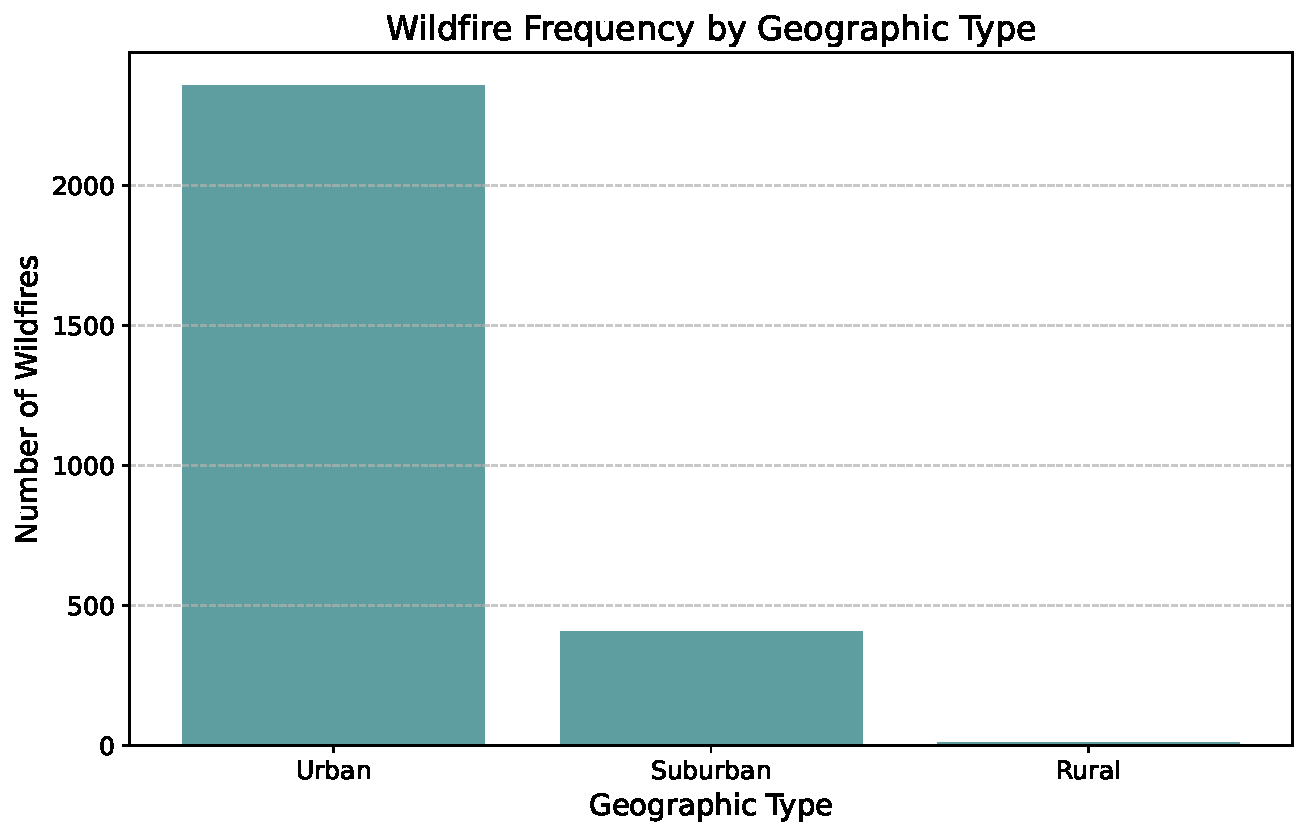
\includegraphics{Final Code_files/figure-pdf/cell-7-output-2.pdf}

\begin{Shaded}
\begin{Highlighting}[]
\NormalTok{population\_data\_path }\OperatorTok{=} \StringTok{\textquotesingle{}/Users/kevinxu/Desktop/Final Project Raw Data/Census\_with\_types.csv\textquotesingle{}}
\NormalTok{firedamage\_data\_path }\OperatorTok{=} \StringTok{\textquotesingle{}/Users/kevinxu/Desktop/Final Project Raw Data/POSTFIRE\_MASTER\_DATA\_SHARE\_2064760709534146017.csv\textquotesingle{}}
\NormalTok{population\_data }\OperatorTok{=}\NormalTok{ pd.read\_csv(population\_data\_path)}
\NormalTok{firedamage\_data }\OperatorTok{=}\NormalTok{ pd.read\_csv(firedamage\_data\_path)}

\NormalTok{population\_data.head(), firedamage\_data.head()}
\NormalTok{population\_data[}\StringTok{"Geography"}\NormalTok{] }\OperatorTok{=}\NormalTok{ (}
\NormalTok{    population\_data[}\StringTok{"Geography"}\NormalTok{]}
\NormalTok{    .}\BuiltInTok{str}\NormalTok{.replace(}\VerbatimStringTok{r"\textbackslash{}s*City\textbackslash{}s*$"}\NormalTok{, }\StringTok{""}\NormalTok{, regex}\OperatorTok{=}\VariableTok{True}\NormalTok{, case}\OperatorTok{=}\VariableTok{False}\NormalTok{)}
\NormalTok{    .}\BuiltInTok{str}\NormalTok{.strip()}
\NormalTok{)}

\BuiltInTok{print}\NormalTok{(population\_data[}\StringTok{"Geography"}\NormalTok{].unique()[:}\DecValTok{10}\NormalTok{])}
\NormalTok{population\_data.head()}
\end{Highlighting}
\end{Shaded}

\begin{verbatim}
['California' 'Alameda County' 'Alameda' 'Albany' 'Ashland CDP' 'Berkeley'
 'Castro Valley CDP' 'Cherryland CDP' 'Dublin' 'Emeryville']
\end{verbatim}

\begin{verbatim}
/var/folders/r4/x5b99tvj66zcn_88m3jn4r6w0000gn/T/ipykernel_22943/3288246651.py:4: DtypeWarning:

Columns (12,36) have mixed types. Specify dtype option on import or set low_memory=False.
\end{verbatim}

\begin{longtable}[]{@{}llllllll@{}}
\toprule\noalign{}
& Geography & Total Population & Land Area in Square Miles & Population
Per Square Mile (Land Area) & Unnamed: 4 & Geoid & geographic type \\
\midrule\noalign{}
\endhead
\bottomrule\noalign{}
\endlastfoot
0 & California & 39538223 & 155858.326771 & 253.680530 & NaN &
0400000US06 & Urban \\
1 & Alameda County & 1682353 & 737.461854 & 2281.274605 & NaN &
0500000US06001 & Urban \\
2 & Alameda & 78280 & 10.448679 & 7491.856487 & NaN & 1600000US0600562 &
Urban \\
3 & Albany & 20271 & 1.789982 & 11324.694641 & NaN & 1600000US0600674 &
Suburban \\
4 & Ashland CDP & 23823 & 1.842571 & 12929.213531 & NaN &
1600000US0602980 & Suburban \\
\end{longtable}

\begin{Shaded}
\begin{Highlighting}[]
\NormalTok{firedamage\_data[}\StringTok{"* City"}\NormalTok{] }\OperatorTok{=}\NormalTok{ (}
\NormalTok{    firedamage\_data[}\StringTok{"* City"}\NormalTok{]}
    \CommentTok{\# Removes "City" regardless of case}
\NormalTok{    .}\BuiltInTok{str}\NormalTok{.replace(}\VerbatimStringTok{r"\textbackslash{}s*City\textbackslash{}s*$"}\NormalTok{, }\StringTok{""}\NormalTok{, regex}\OperatorTok{=}\VariableTok{True}\NormalTok{, case}\OperatorTok{=}\VariableTok{False}\NormalTok{)}
\NormalTok{    .}\BuiltInTok{str}\NormalTok{.strip()  }\CommentTok{\# Removes leading/trailing whitespace}
\NormalTok{)}

\CommentTok{\# Verify the changes}
\CommentTok{\# Display unique values to confirm "City" is removed}
\NormalTok{firedamage\_data[}\StringTok{"* City"}\NormalTok{].unique()[:}\DecValTok{10}\NormalTok{]}
\NormalTok{firedamage\_data.head()}
\end{Highlighting}
\end{Shaded}

\begin{longtable}[]{@{}llllllllllllllllllllll@{}}
\toprule\noalign{}
& OBJECTID & * Damage & * Street Number & * Street Name & * Street Type
(e.g. road, drive, lane, etc.) & Street Suffix (e.g. apt. 23, blding C)
& * City & State & Zip Code & * CAL FIRE Unit & ... & Fire Name
(Secondary) & APN (parcel) & Assessed Improved Value (parcel) & Year
Built (parcel) & Site Address (parcel) & GLOBALID & Latitude & Longitude
& x & y \\
\midrule\noalign{}
\endhead
\bottomrule\noalign{}
\endlastfoot
0 & 1 & No Damage & 8376.0 & Quail Canyon & Road & NaN & Winters & CA &
NaN & LNU & ... & Quail & 101090290 & 510000.0 & 1997.0 & 8376 QUAIL
CANYON RD VACAVILLE CA 95688 & e1919a06-b4c6-476d-99e5-f0b45b070de8 &
38.474960 & -122.044465 & -1.358593e+07 & 4.646741e+06 \\
1 & 2 & Affected (1-9\%) & 8402.0 & Quail Canyon & Road & NaN & Winters
& CA & NaN & LNU & ... & Quail & 101090270 & 573052.0 & 1980.0 & 8402
QUAIL CANYON RD VACAVILLE CA 95688 &
b090eeb6-5b18-421e-9723-af7c9144587c & 38.477442 & -122.043252 &
-1.358579e+07 & 4.647094e+06 \\
2 & 3 & No Damage & 8430.0 & Quail Canyon & Road & NaN & Winters & CA &
NaN & LNU & ... & Quail & 101090310 & 350151.0 & 2004.0 & 8430 QUAIL
CANYON RD VACAVILLE CA 95688 & 268da70b-753f-46aa-8fb1-327099337395 &
38.479358 & -122.044585 & -1.358594e+07 & 4.647366e+06 \\
3 & 4 & No Damage & 3838.0 & Putah Creek & Road & NaN & Winters & CA &
NaN & LNU & ... & Quail & 103010240 & 134880.0 & 1981.0 & 3838 PUTAH
CREEK RD WINTERS CA 95694 & 64d4a278-5ee9-414a-8bf4-247c5b5c60f9 &
38.487313 & -122.015115 & -1.358266e+07 & 4.648497e+06 \\
4 & 5 & No Damage & 3830.0 & Putah Creek & Road & NaN & Winters & CA &
NaN & LNU & ... & Quail & 103010220 & 346648.0 & 1980.0 & 3830 PUTAH
CREEK RD WINTERS CA 95694 & 1b44b214-01fd-4f06-b764-eb42a1ec93d7 &
38.485636 & -122.016122 & -1.358277e+07 & 4.648259e+06 \\
\end{longtable}

\begin{Shaded}
\begin{Highlighting}[]
\CommentTok{\# Remove rows where Geography or * City contains "County" in either dataset}
\NormalTok{population\_data\_cleaned }\OperatorTok{=}\NormalTok{ population\_data[}\OperatorTok{\textasciitilde{}}\NormalTok{population\_data[}\StringTok{"Geography"}\NormalTok{].}\BuiltInTok{str}\NormalTok{.contains(}
    \StringTok{"County"}\NormalTok{, case}\OperatorTok{=}\VariableTok{False}\NormalTok{, na}\OperatorTok{=}\VariableTok{False}\NormalTok{)]}
\NormalTok{firedamage\_data\_cleaned }\OperatorTok{=}\NormalTok{ firedamage\_data[}\OperatorTok{\textasciitilde{}}\NormalTok{firedamage\_data[}\StringTok{"* City"}\NormalTok{].}\BuiltInTok{str}\NormalTok{.contains(}
    \StringTok{"County"}\NormalTok{, case}\OperatorTok{=}\VariableTok{False}\NormalTok{, na}\OperatorTok{=}\VariableTok{False}\NormalTok{)]}

\CommentTok{\# Standardize column names for merging}
\NormalTok{population\_data\_cleaned }\OperatorTok{=}\NormalTok{ population\_data\_cleaned.rename(}
\NormalTok{    columns}\OperatorTok{=}\NormalTok{\{}\StringTok{"Geography"}\NormalTok{: }\StringTok{"City"}\NormalTok{\})}
\NormalTok{firedamage\_data\_cleaned }\OperatorTok{=}\NormalTok{ firedamage\_data\_cleaned.rename(}
\NormalTok{    columns}\OperatorTok{=}\NormalTok{\{}\StringTok{"* City"}\NormalTok{: }\StringTok{"City"}\NormalTok{\})}

\CommentTok{\# Merge the datasets based on the City column}
\NormalTok{merged\_data }\OperatorTok{=}\NormalTok{ pd.merge(}
\NormalTok{    firedamage\_data\_cleaned,}
\NormalTok{    population\_data\_cleaned,}
\NormalTok{    on}\OperatorTok{=}\StringTok{"City"}\NormalTok{,}
\NormalTok{    how}\OperatorTok{=}\StringTok{"inner"}
\NormalTok{)}

\CommentTok{\# Display the first few rows of the merged dataset to confirm}
\NormalTok{merged\_data.head()}
\end{Highlighting}
\end{Shaded}

\begin{longtable}[]{@{}llllllllllllllllllllll@{}}
\toprule\noalign{}
& OBJECTID & * Damage & * Street Number & * Street Name & * Street Type
(e.g. road, drive, lane, etc.) & Street Suffix (e.g. apt. 23, blding C)
& City & State & Zip Code & * CAL FIRE Unit & ... & Latitude & Longitude
& x & y & Total Population & Land Area in Square Miles & Population Per
Square Mile (Land Area) & Unnamed: 4 & Geoid & geographic type \\
\midrule\noalign{}
\endhead
\bottomrule\noalign{}
\endlastfoot
0 & 1 & No Damage & 8376.0 & Quail Canyon & Road & NaN & Winters & CA &
NaN & LNU & ... & 38.474960 & -122.044465 & -1.358593e+07 & 4.646741e+06
& 7115 & 2.934826 & 2424.334246 & NaN & 1600000US0686034 & Suburban \\
1 & 2 & Affected (1-9\%) & 8402.0 & Quail Canyon & Road & NaN & Winters
& CA & NaN & LNU & ... & 38.477442 & -122.043252 & -1.358579e+07 &
4.647094e+06 & 7115 & 2.934826 & 2424.334246 & NaN & 1600000US0686034 &
Suburban \\
2 & 3 & No Damage & 8430.0 & Quail Canyon & Road & NaN & Winters & CA &
NaN & LNU & ... & 38.479358 & -122.044585 & -1.358594e+07 & 4.647366e+06
& 7115 & 2.934826 & 2424.334246 & NaN & 1600000US0686034 & Suburban \\
3 & 4 & No Damage & 3838.0 & Putah Creek & Road & NaN & Winters & CA &
NaN & LNU & ... & 38.487313 & -122.015115 & -1.358266e+07 & 4.648497e+06
& 7115 & 2.934826 & 2424.334246 & NaN & 1600000US0686034 & Suburban \\
4 & 5 & No Damage & 3830.0 & Putah Creek & Road & NaN & Winters & CA &
NaN & LNU & ... & 38.485636 & -122.016122 & -1.358277e+07 & 4.648259e+06
& 7115 & 2.934826 & 2424.334246 & NaN & 1600000US0686034 & Suburban \\
\end{longtable}

\section{bar plot of 2020 (done by Regina
Hou)}\label{bar-plot-of-2020-done-by-regina-hou}

\begin{Shaded}
\begin{Highlighting}[]
\CommentTok{\# Filter for 2020 data only after merging}
\NormalTok{merged\_data[}\StringTok{"Year"}\NormalTok{] }\OperatorTok{=}\NormalTok{ pd.to\_datetime(}
\NormalTok{    merged\_data[}\StringTok{"Incident Start Date"}\NormalTok{], errors}\OperatorTok{=}\StringTok{"coerce"}\NormalTok{).dt.year}
\NormalTok{merged\_data\_2020 }\OperatorTok{=}\NormalTok{ merged\_data[merged\_data[}\StringTok{"Year"}\NormalTok{] }\OperatorTok{==} \DecValTok{2020}\NormalTok{]}
\end{Highlighting}
\end{Shaded}

\begin{verbatim}
/var/folders/r4/x5b99tvj66zcn_88m3jn4r6w0000gn/T/ipykernel_22943/454140121.py:2: UserWarning:

Could not infer format, so each element will be parsed individually, falling back to `dateutil`. To ensure parsing is consistent and as-expected, please specify a format.
\end{verbatim}

\begin{Shaded}
\begin{Highlighting}[]
\CommentTok{\# Filter for 2020 data only after merging and exclude "No Damage"}
\ImportTok{from}\NormalTok{ matplotlib.lines }\ImportTok{import}\NormalTok{ Line2D}
\NormalTok{merged\_data[}\StringTok{"Year"}\NormalTok{] }\OperatorTok{=}\NormalTok{ pd.to\_datetime(}
\NormalTok{    merged\_data[}\StringTok{"Incident Start Date"}\NormalTok{], errors}\OperatorTok{=}\StringTok{"coerce"}\NormalTok{).dt.year}
\NormalTok{merged\_data\_2020 }\OperatorTok{=}\NormalTok{ merged\_data[}
\NormalTok{    (merged\_data[}\StringTok{"Year"}\NormalTok{] }\OperatorTok{==} \DecValTok{2020}\NormalTok{) }\OperatorTok{\&}
\NormalTok{    (merged\_data[}\StringTok{"* Damage"}\NormalTok{] }\OperatorTok{!=} \StringTok{"No Damage"}\NormalTok{)}
\NormalTok{]}

\CommentTok{\# Group data by geographic type and damage level, and count occurrences}
\NormalTok{damage\_counts\_2020 }\OperatorTok{=}\NormalTok{ (}
\NormalTok{    merged\_data\_2020.groupby([}\StringTok{"geographic type"}\NormalTok{, }\StringTok{"* Damage"}\NormalTok{])}
\NormalTok{    .size()}
\NormalTok{    .reset\_index(name}\OperatorTok{=}\StringTok{"Count"}\NormalTok{)}
\NormalTok{)}

\CommentTok{\# Define the order of damage levels}
\NormalTok{damage\_order }\OperatorTok{=}\NormalTok{ [}
    \StringTok{"Affected (1{-}9\%)"}\NormalTok{,}
    \StringTok{"Minor (10{-}25\%)"}\NormalTok{,}
    \StringTok{"Major (26{-}50\%)"}\NormalTok{,}
    \StringTok{"Destroyed (\textgreater{}50\%)"}
\NormalTok{]}

\CommentTok{\# Update damage levels for sorting and visualization}
\NormalTok{damage\_counts\_2020[}\StringTok{"* Damage"}\NormalTok{] }\OperatorTok{=}\NormalTok{ pd.Categorical(}
\NormalTok{    damage\_counts\_2020[}\StringTok{"* Damage"}\NormalTok{], categories}\OperatorTok{=}\NormalTok{damage\_order, ordered}\OperatorTok{=}\VariableTok{True}
\NormalTok{)}

\CommentTok{\# Sort the data by Geographic Type and Damage Level}
\NormalTok{damage\_counts\_2020 }\OperatorTok{=}\NormalTok{ damage\_counts\_2020.sort\_values(}
\NormalTok{    by}\OperatorTok{=}\NormalTok{[}\StringTok{"geographic type"}\NormalTok{, }\StringTok{"* Damage"}\NormalTok{])}

\CommentTok{\# Create a new x{-}axis label with rearranged categories}
\NormalTok{damage\_counts\_2020[}\StringTok{"Label"}\NormalTok{] }\OperatorTok{=}\NormalTok{ (}
\NormalTok{    damage\_counts\_2020[}\StringTok{"geographic type"}\NormalTok{] }\OperatorTok{+} \StringTok{" + "} \OperatorTok{+}
\NormalTok{    damage\_counts\_2020[}\StringTok{"* Damage"}\NormalTok{].astype(}\BuiltInTok{str}\NormalTok{)}
\NormalTok{)}

\CommentTok{\# Assign colors based on geographic type}
\NormalTok{colors }\OperatorTok{=}\NormalTok{ \{}\StringTok{"Rural"}\NormalTok{: }\StringTok{"green"}\NormalTok{, }\StringTok{"Suburban"}\NormalTok{: }\StringTok{"orange"}\NormalTok{, }\StringTok{"Urban"}\NormalTok{: }\StringTok{"red"}\NormalTok{\}}
\NormalTok{damage\_counts\_2020[}\StringTok{"Bar Color"}\NormalTok{] }\OperatorTok{=}\NormalTok{ damage\_counts\_2020[}\StringTok{"geographic type"}\NormalTok{].}\BuiltInTok{map}\NormalTok{(}
\NormalTok{    colors)}

\CommentTok{\# Plot the bar chart}
\NormalTok{plt.figure(figsize}\OperatorTok{=}\NormalTok{(}\DecValTok{14}\NormalTok{, }\DecValTok{8}\NormalTok{))}
\NormalTok{bars }\OperatorTok{=}\NormalTok{ plt.bar(}
\NormalTok{    damage\_counts\_2020[}\StringTok{"Label"}\NormalTok{],}
\NormalTok{    damage\_counts\_2020[}\StringTok{"Count"}\NormalTok{],}
\NormalTok{    color}\OperatorTok{=}\NormalTok{damage\_counts\_2020[}\StringTok{"Bar Color"}\NormalTok{],}
\NormalTok{)}

\CommentTok{\# Add counts on top of each bar}
\ControlFlowTok{for}\NormalTok{ bar }\KeywordTok{in}\NormalTok{ bars:}
\NormalTok{    yval }\OperatorTok{=}\NormalTok{ bar.get\_height()}
\NormalTok{    plt.text(bar.get\_x() }\OperatorTok{+}\NormalTok{ bar.get\_width() }\OperatorTok{/} \DecValTok{2}\NormalTok{, yval }\OperatorTok{+} \FloatTok{0.5}\NormalTok{,}
             \BuiltInTok{int}\NormalTok{(yval), ha}\OperatorTok{=}\StringTok{"center"}\NormalTok{, va}\OperatorTok{=}\StringTok{"bottom"}\NormalTok{, fontsize}\OperatorTok{=}\DecValTok{10}\NormalTok{)}

\CommentTok{\# Customize the chart}
\NormalTok{plt.title(}\StringTok{"Fire Damage Counts by Geographic Type and Damage Level (2020, Excluding No Damage)"}\NormalTok{, fontsize}\OperatorTok{=}\DecValTok{16}\NormalTok{)}
\NormalTok{plt.xlabel(}\StringTok{"Geographic Type + Damage Level"}\NormalTok{, fontsize}\OperatorTok{=}\DecValTok{12}\NormalTok{)}
\NormalTok{plt.ylabel(}\StringTok{"Counts"}\NormalTok{, fontsize}\OperatorTok{=}\DecValTok{12}\NormalTok{)}
\NormalTok{plt.xticks(rotation}\OperatorTok{=}\DecValTok{45}\NormalTok{, ha}\OperatorTok{=}\StringTok{"right"}\NormalTok{, fontsize}\OperatorTok{=}\DecValTok{10}\NormalTok{)}

\CommentTok{\# Add a legend for the bar colors}

\NormalTok{legend\_elements }\OperatorTok{=}\NormalTok{ [}
\NormalTok{    Line2D([}\DecValTok{0}\NormalTok{], [}\DecValTok{0}\NormalTok{], color}\OperatorTok{=}\StringTok{"green"}\NormalTok{, lw}\OperatorTok{=}\DecValTok{6}\NormalTok{, label}\OperatorTok{=}\StringTok{"Rural"}\NormalTok{),}
\NormalTok{    Line2D([}\DecValTok{0}\NormalTok{], [}\DecValTok{0}\NormalTok{], color}\OperatorTok{=}\StringTok{"orange"}\NormalTok{, lw}\OperatorTok{=}\DecValTok{6}\NormalTok{, label}\OperatorTok{=}\StringTok{"Suburban"}\NormalTok{),}
\NormalTok{    Line2D([}\DecValTok{0}\NormalTok{], [}\DecValTok{0}\NormalTok{], color}\OperatorTok{=}\StringTok{"red"}\NormalTok{, lw}\OperatorTok{=}\DecValTok{6}\NormalTok{, label}\OperatorTok{=}\StringTok{"Urban"}\NormalTok{),}
\NormalTok{]}

\NormalTok{plt.legend(handles}\OperatorTok{=}\NormalTok{legend\_elements, title}\OperatorTok{=}\StringTok{"Geographic Type"}\NormalTok{,}
\NormalTok{           loc}\OperatorTok{=}\StringTok{"upper right"}\NormalTok{, fontsize}\OperatorTok{=}\DecValTok{10}\NormalTok{)}

\NormalTok{plt.tight\_layout()}

\CommentTok{\# Show the plot}
\NormalTok{plt.show()}
\end{Highlighting}
\end{Shaded}

\begin{verbatim}
/var/folders/r4/x5b99tvj66zcn_88m3jn4r6w0000gn/T/ipykernel_22943/1844741617.py:3: UserWarning:

Could not infer format, so each element will be parsed individually, falling back to `dateutil`. To ensure parsing is consistent and as-expected, please specify a format.
\end{verbatim}

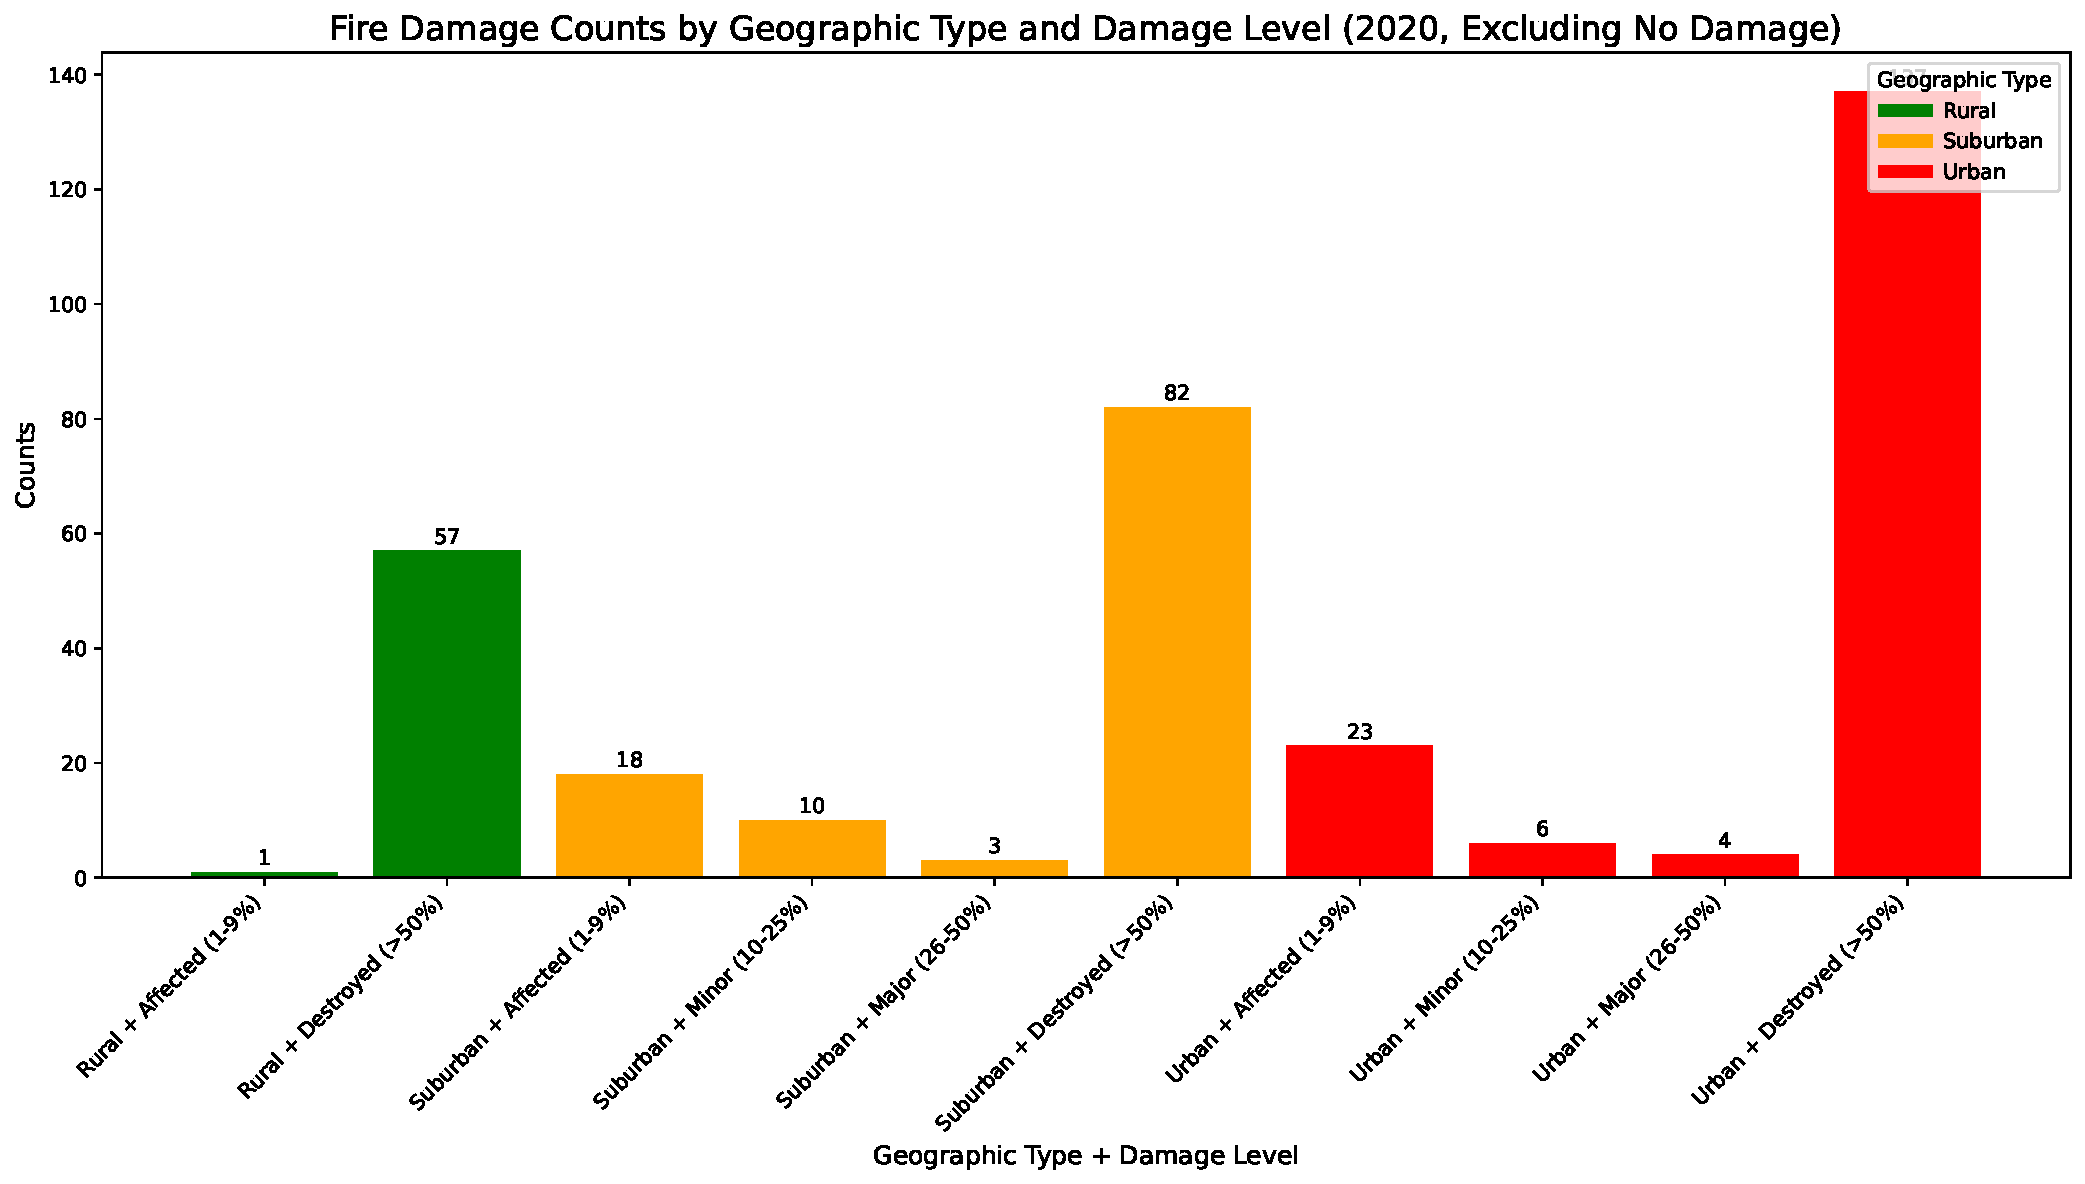
\includegraphics{Final Code_files/figure-pdf/cell-12-output-2.pdf}

\section{plot of 2021 (done by Regina
Hou)}\label{plot-of-2021-done-by-regina-hou}

\begin{Shaded}
\begin{Highlighting}[]
\CommentTok{\# Filter for 2021 data only after merging}
\NormalTok{merged\_data\_2021 }\OperatorTok{=}\NormalTok{ merged\_data[}
\NormalTok{    (merged\_data[}\StringTok{"Year"}\NormalTok{] }\OperatorTok{==} \DecValTok{2021}\NormalTok{) }\OperatorTok{\&} 
\NormalTok{    (}\OperatorTok{\textasciitilde{}}\NormalTok{merged\_data[}\StringTok{"* Damage"}\NormalTok{].isna()) }\OperatorTok{\&} 
\NormalTok{    (}\OperatorTok{\textasciitilde{}}\NormalTok{merged\_data[}\StringTok{"geographic type"}\NormalTok{].isna())}
\NormalTok{].copy()}

\CommentTok{\# Verify that there are no NaN values remaining}
\BuiltInTok{print}\NormalTok{(}\StringTok{"NaN values in geographic type:"}\NormalTok{, merged\_data\_2021[}\StringTok{"geographic type"}\NormalTok{].isna().}\BuiltInTok{sum}\NormalTok{())}
\BuiltInTok{print}\NormalTok{(}\StringTok{"NaN values in * Damage:"}\NormalTok{, merged\_data\_2021[}\StringTok{"* Damage"}\NormalTok{].isna().}\BuiltInTok{sum}\NormalTok{())}
\end{Highlighting}
\end{Shaded}

\begin{verbatim}
NaN values in geographic type: 0
NaN values in * Damage: 0
\end{verbatim}

\begin{Shaded}
\begin{Highlighting}[]
\CommentTok{\# Filter for 2021 data only after merging and exclude "No Damage"}
\NormalTok{merged\_data\_2021 }\OperatorTok{=}\NormalTok{ merged\_data[}
\NormalTok{    (merged\_data[}\StringTok{"Year"}\NormalTok{] }\OperatorTok{==} \DecValTok{2021}\NormalTok{) }\OperatorTok{\&}
\NormalTok{    (merged\_data[}\StringTok{"* Damage"}\NormalTok{] }\OperatorTok{!=} \StringTok{"No Damage"}\NormalTok{)}
\NormalTok{]}

\CommentTok{\# Group data by geographic type and damage level, and count occurrences}
\NormalTok{damage\_counts\_2021 }\OperatorTok{=}\NormalTok{ (}
\NormalTok{    merged\_data\_2021.groupby([}\StringTok{"geographic type"}\NormalTok{, }\StringTok{"* Damage"}\NormalTok{])}
\NormalTok{    .size()}
\NormalTok{    .reset\_index(name}\OperatorTok{=}\StringTok{"Count"}\NormalTok{)}
\NormalTok{)}

\CommentTok{\# Define the order of damage levels}
\NormalTok{damage\_order }\OperatorTok{=}\NormalTok{ [}
    \StringTok{"Affected (1{-}9\%)"}\NormalTok{, }
    \StringTok{"Minor (10{-}25\%)"}\NormalTok{, }
    \StringTok{"Major (26{-}50\%)"}\NormalTok{, }
    \StringTok{"Destroyed (\textgreater{}50\%)"}
\NormalTok{]}

\CommentTok{\# Update damage levels for sorting and visualization}
\NormalTok{damage\_counts\_2021[}\StringTok{"* Damage"}\NormalTok{] }\OperatorTok{=}\NormalTok{ pd.Categorical(}
\NormalTok{    damage\_counts\_2021[}\StringTok{"* Damage"}\NormalTok{], categories}\OperatorTok{=}\NormalTok{damage\_order, ordered}\OperatorTok{=}\VariableTok{True}
\NormalTok{)}

\CommentTok{\# Sort the data by Geographic Type and Damage Level}
\NormalTok{damage\_counts\_2021 }\OperatorTok{=}\NormalTok{ damage\_counts\_2021.sort\_values(by}\OperatorTok{=}\NormalTok{[}\StringTok{"geographic type"}\NormalTok{, }\StringTok{"* Damage"}\NormalTok{])}

\CommentTok{\# Create a new x{-}axis label with rearranged categories}
\NormalTok{damage\_counts\_2021[}\StringTok{"Label"}\NormalTok{] }\OperatorTok{=}\NormalTok{ (}
\NormalTok{    damage\_counts\_2021[}\StringTok{"geographic type"}\NormalTok{] }\OperatorTok{+} \StringTok{" + "} \OperatorTok{+}\NormalTok{ damage\_counts\_2021[}\StringTok{"* Damage"}\NormalTok{].astype(}\BuiltInTok{str}\NormalTok{)}
\NormalTok{)}

\CommentTok{\# Assign colors based on geographic type}
\NormalTok{colors }\OperatorTok{=}\NormalTok{ \{}\StringTok{"Rural"}\NormalTok{: }\StringTok{"green"}\NormalTok{, }\StringTok{"Suburban"}\NormalTok{: }\StringTok{"orange"}\NormalTok{, }\StringTok{"Urban"}\NormalTok{: }\StringTok{"red"}\NormalTok{\}}
\NormalTok{damage\_counts\_2021[}\StringTok{"Bar Color"}\NormalTok{] }\OperatorTok{=}\NormalTok{ damage\_counts\_2021[}\StringTok{"geographic type"}\NormalTok{].}\BuiltInTok{map}\NormalTok{(colors)}

\CommentTok{\# Plot the bar chart}
\NormalTok{plt.figure(figsize}\OperatorTok{=}\NormalTok{(}\DecValTok{14}\NormalTok{, }\DecValTok{8}\NormalTok{))}
\NormalTok{bars }\OperatorTok{=}\NormalTok{ plt.bar(}
\NormalTok{    damage\_counts\_2021[}\StringTok{"Label"}\NormalTok{],}
\NormalTok{    damage\_counts\_2021[}\StringTok{"Count"}\NormalTok{],}
\NormalTok{    color}\OperatorTok{=}\NormalTok{damage\_counts\_2021[}\StringTok{"Bar Color"}\NormalTok{],}
\NormalTok{)}

\CommentTok{\# Add counts on top of each bar}
\ControlFlowTok{for}\NormalTok{ bar }\KeywordTok{in}\NormalTok{ bars:}
\NormalTok{    yval }\OperatorTok{=}\NormalTok{ bar.get\_height()}
\NormalTok{    plt.text(bar.get\_x() }\OperatorTok{+}\NormalTok{ bar.get\_width() }\OperatorTok{/} \DecValTok{2}\NormalTok{, yval }\OperatorTok{+} \FloatTok{0.5}\NormalTok{, }\BuiltInTok{int}\NormalTok{(yval), ha}\OperatorTok{=}\StringTok{"center"}\NormalTok{, va}\OperatorTok{=}\StringTok{"bottom"}\NormalTok{, fontsize}\OperatorTok{=}\DecValTok{10}\NormalTok{)}

\CommentTok{\# Customize the chart}
\NormalTok{plt.title(}\StringTok{"Fire Damage Counts by Geographic Type and Damage Level (2021, Excluding No Damage)"}\NormalTok{, fontsize}\OperatorTok{=}\DecValTok{16}\NormalTok{)}
\NormalTok{plt.xlabel(}\StringTok{"Geographic Type + Damage Level"}\NormalTok{, fontsize}\OperatorTok{=}\DecValTok{12}\NormalTok{)}
\NormalTok{plt.ylabel(}\StringTok{"Counts"}\NormalTok{, fontsize}\OperatorTok{=}\DecValTok{12}\NormalTok{)}
\NormalTok{plt.xticks(rotation}\OperatorTok{=}\DecValTok{45}\NormalTok{, ha}\OperatorTok{=}\StringTok{"right"}\NormalTok{, fontsize}\OperatorTok{=}\DecValTok{10}\NormalTok{)}

\CommentTok{\# Add a legend for the bar colors}
\ImportTok{from}\NormalTok{ matplotlib.lines }\ImportTok{import}\NormalTok{ Line2D}

\NormalTok{legend\_elements }\OperatorTok{=}\NormalTok{ [}
\NormalTok{    Line2D([}\DecValTok{0}\NormalTok{], [}\DecValTok{0}\NormalTok{], color}\OperatorTok{=}\StringTok{"green"}\NormalTok{, lw}\OperatorTok{=}\DecValTok{6}\NormalTok{, label}\OperatorTok{=}\StringTok{"Rural"}\NormalTok{),}
\NormalTok{    Line2D([}\DecValTok{0}\NormalTok{], [}\DecValTok{0}\NormalTok{], color}\OperatorTok{=}\StringTok{"orange"}\NormalTok{, lw}\OperatorTok{=}\DecValTok{6}\NormalTok{, label}\OperatorTok{=}\StringTok{"Suburban"}\NormalTok{),}
\NormalTok{    Line2D([}\DecValTok{0}\NormalTok{], [}\DecValTok{0}\NormalTok{], color}\OperatorTok{=}\StringTok{"red"}\NormalTok{, lw}\OperatorTok{=}\DecValTok{6}\NormalTok{, label}\OperatorTok{=}\StringTok{"Urban"}\NormalTok{),}
\NormalTok{]}

\NormalTok{plt.legend(handles}\OperatorTok{=}\NormalTok{legend\_elements, title}\OperatorTok{=}\StringTok{"Geographic Type"}\NormalTok{, loc}\OperatorTok{=}\StringTok{"upper right"}\NormalTok{, fontsize}\OperatorTok{=}\DecValTok{10}\NormalTok{)}

\NormalTok{plt.tight\_layout()}

\CommentTok{\# Show the plot}
\NormalTok{plt.show()}
\end{Highlighting}
\end{Shaded}

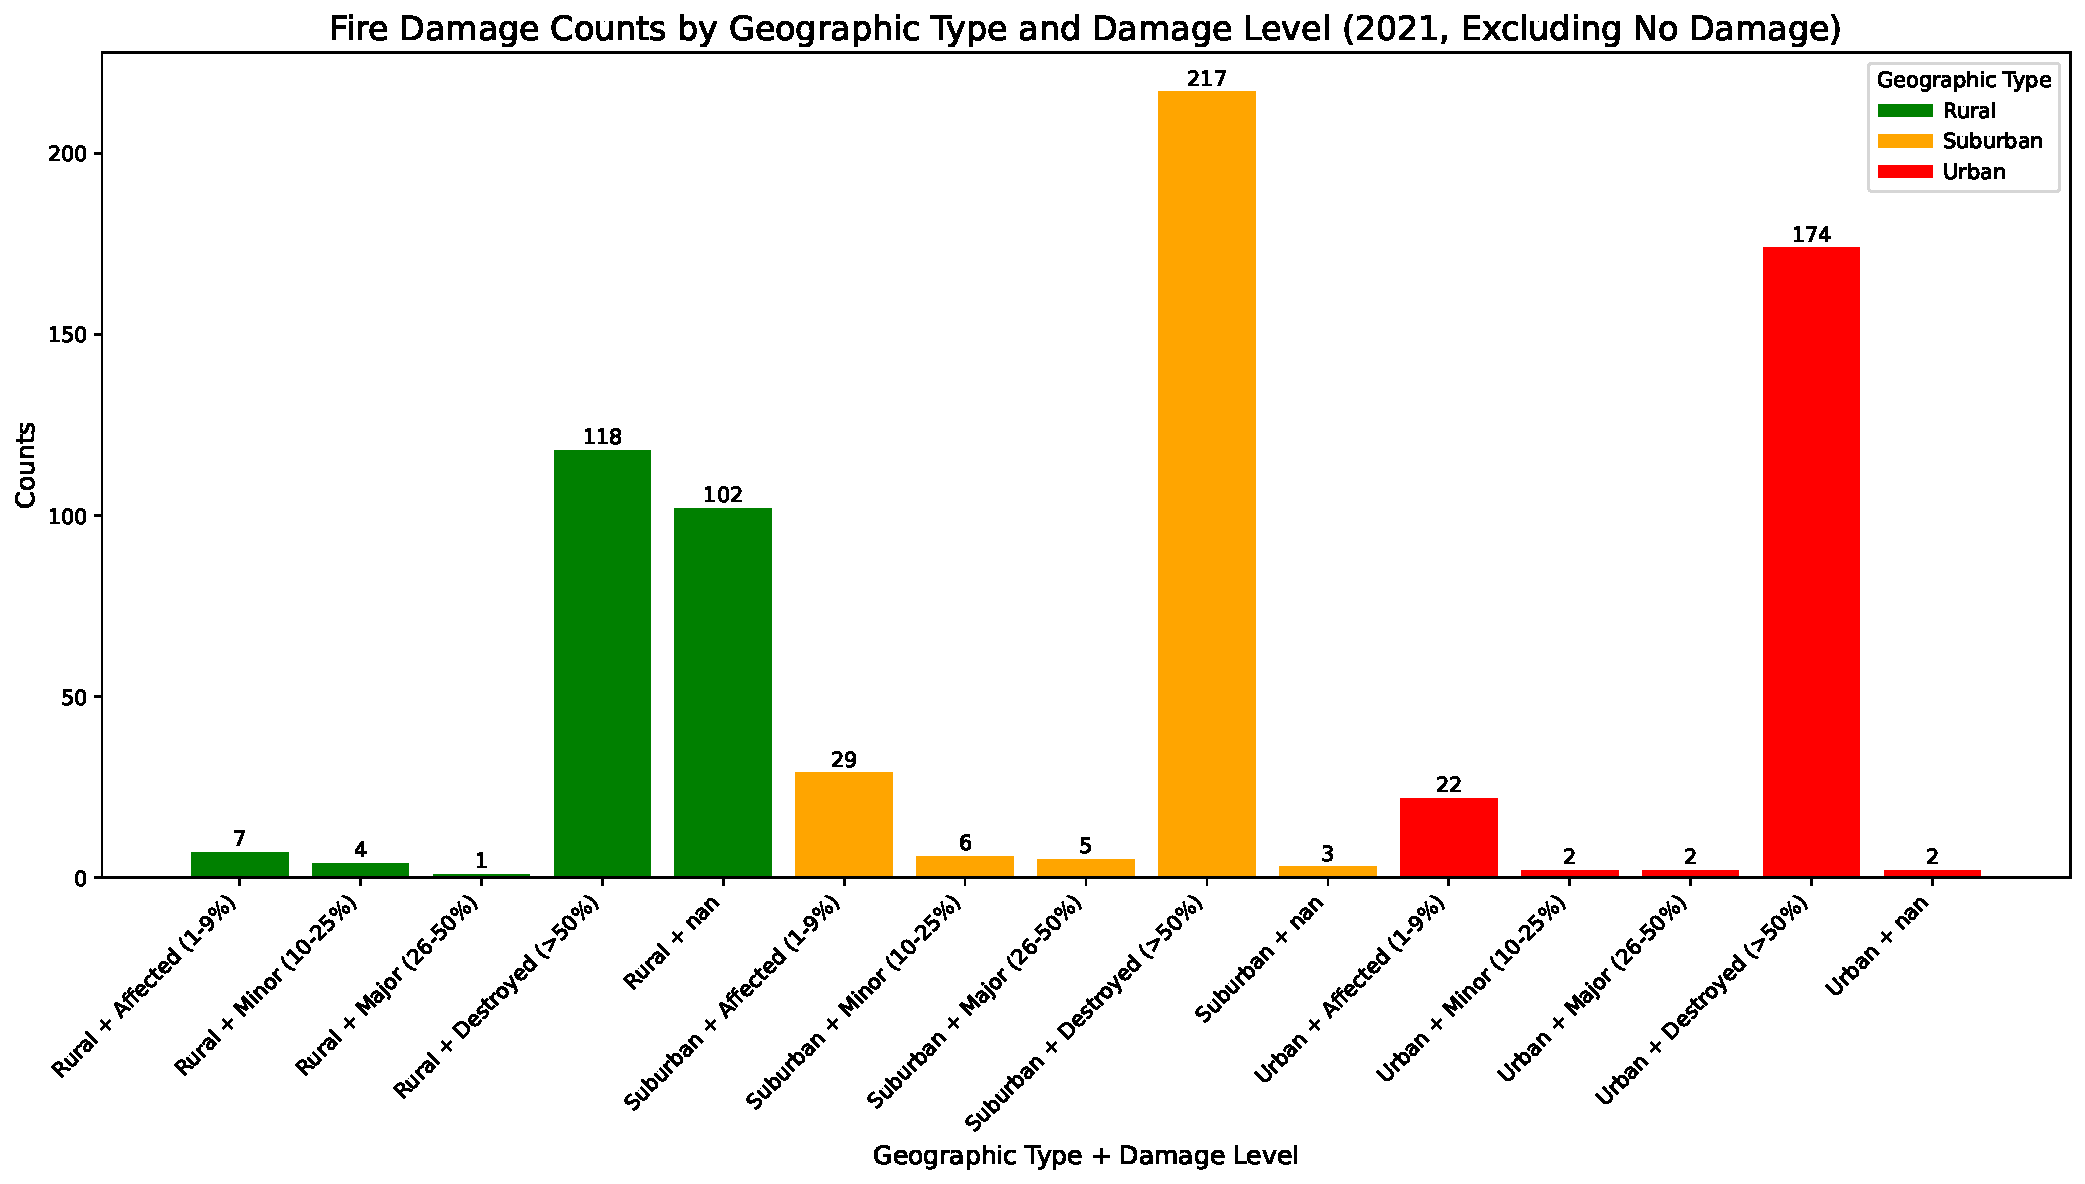
\includegraphics{Final Code_files/figure-pdf/cell-14-output-1.pdf}

\section{plot of 2022 (done by Regina
Hou)}\label{plot-of-2022-done-by-regina-hou}

\begin{Shaded}
\begin{Highlighting}[]
\CommentTok{\# Filter for 2022 data only after merging}
\NormalTok{merged\_data[}\StringTok{"Year"}\NormalTok{] }\OperatorTok{=}\NormalTok{ pd.to\_datetime(merged\_data[}\StringTok{"Incident Start Date"}\NormalTok{], errors}\OperatorTok{=}\StringTok{"coerce"}\NormalTok{).dt.year}
\NormalTok{merged\_data\_2022 }\OperatorTok{=}\NormalTok{ merged\_data[merged\_data[}\StringTok{"Year"}\NormalTok{] }\OperatorTok{==} \DecValTok{2022}\NormalTok{]}
\end{Highlighting}
\end{Shaded}

\begin{verbatim}
/var/folders/r4/x5b99tvj66zcn_88m3jn4r6w0000gn/T/ipykernel_22943/3282159924.py:2: UserWarning:

Could not infer format, so each element will be parsed individually, falling back to `dateutil`. To ensure parsing is consistent and as-expected, please specify a format.
\end{verbatim}

\begin{Shaded}
\begin{Highlighting}[]
\CommentTok{\# Filter for 2022 data only after merging and exclude "No Damage"}
\NormalTok{merged\_data\_2022 }\OperatorTok{=}\NormalTok{ merged\_data[}
\NormalTok{    (merged\_data[}\StringTok{"Year"}\NormalTok{] }\OperatorTok{==} \DecValTok{2022}\NormalTok{) }\OperatorTok{\&}
\NormalTok{    (merged\_data[}\StringTok{"* Damage"}\NormalTok{] }\OperatorTok{!=} \StringTok{"No Damage"}\NormalTok{)}
\NormalTok{]}

\CommentTok{\# Group data by geographic type and damage level, and count occurrences}
\NormalTok{damage\_counts\_2022 }\OperatorTok{=}\NormalTok{ (}
\NormalTok{    merged\_data\_2022.groupby([}\StringTok{"geographic type"}\NormalTok{, }\StringTok{"* Damage"}\NormalTok{])}
\NormalTok{    .size()}
\NormalTok{    .reset\_index(name}\OperatorTok{=}\StringTok{"Count"}\NormalTok{)}
\NormalTok{)}

\CommentTok{\# Define the order of damage levels}
\NormalTok{damage\_order }\OperatorTok{=}\NormalTok{ [}
    \StringTok{"Affected (1{-}9\%)"}\NormalTok{, }
    \StringTok{"Minor (10{-}25\%)"}\NormalTok{, }
    \StringTok{"Major (26{-}50\%)"}\NormalTok{, }
    \StringTok{"Destroyed (\textgreater{}50\%)"}
\NormalTok{]}

\CommentTok{\# Update damage levels for sorting and visualization}
\NormalTok{damage\_counts\_2022[}\StringTok{"* Damage"}\NormalTok{] }\OperatorTok{=}\NormalTok{ pd.Categorical(}
\NormalTok{    damage\_counts\_2022[}\StringTok{"* Damage"}\NormalTok{], categories}\OperatorTok{=}\NormalTok{damage\_order, ordered}\OperatorTok{=}\VariableTok{True}
\NormalTok{)}

\CommentTok{\# Sort the data by Geographic Type and Damage Level}
\NormalTok{damage\_counts\_2022 }\OperatorTok{=}\NormalTok{ damage\_counts\_2022.sort\_values(by}\OperatorTok{=}\NormalTok{[}\StringTok{"geographic type"}\NormalTok{, }\StringTok{"* Damage"}\NormalTok{])}

\CommentTok{\# Create a new x{-}axis label with rearranged categories}
\NormalTok{damage\_counts\_2022[}\StringTok{"Label"}\NormalTok{] }\OperatorTok{=}\NormalTok{ (}
\NormalTok{    damage\_counts\_2022[}\StringTok{"geographic type"}\NormalTok{] }\OperatorTok{+} \StringTok{" + "} \OperatorTok{+}\NormalTok{ damage\_counts\_2022[}\StringTok{"* Damage"}\NormalTok{].astype(}\BuiltInTok{str}\NormalTok{)}
\NormalTok{)}

\CommentTok{\# Assign colors based on geographic type}
\NormalTok{colors }\OperatorTok{=}\NormalTok{ \{}\StringTok{"Rural"}\NormalTok{: }\StringTok{"green"}\NormalTok{, }\StringTok{"Suburban"}\NormalTok{: }\StringTok{"orange"}\NormalTok{, }\StringTok{"Urban"}\NormalTok{: }\StringTok{"red"}\NormalTok{\}}
\NormalTok{damage\_counts\_2022[}\StringTok{"Bar Color"}\NormalTok{] }\OperatorTok{=}\NormalTok{ damage\_counts\_2022[}\StringTok{"geographic type"}\NormalTok{].}\BuiltInTok{map}\NormalTok{(colors)}

\CommentTok{\# Plot the bar chart}
\NormalTok{plt.figure(figsize}\OperatorTok{=}\NormalTok{(}\DecValTok{14}\NormalTok{, }\DecValTok{8}\NormalTok{))}
\NormalTok{bars }\OperatorTok{=}\NormalTok{ plt.bar(}
\NormalTok{    damage\_counts\_2022[}\StringTok{"Label"}\NormalTok{],}
\NormalTok{    damage\_counts\_2022[}\StringTok{"Count"}\NormalTok{],}
\NormalTok{    color}\OperatorTok{=}\NormalTok{damage\_counts\_2022[}\StringTok{"Bar Color"}\NormalTok{],}
\NormalTok{)}

\CommentTok{\# Add counts on top of each bar}
\ControlFlowTok{for}\NormalTok{ bar }\KeywordTok{in}\NormalTok{ bars:}
\NormalTok{    yval }\OperatorTok{=}\NormalTok{ bar.get\_height()}
\NormalTok{    plt.text(bar.get\_x() }\OperatorTok{+}\NormalTok{ bar.get\_width() }\OperatorTok{/} \DecValTok{2}\NormalTok{, yval }\OperatorTok{+} \FloatTok{0.5}\NormalTok{, }\BuiltInTok{int}\NormalTok{(yval), ha}\OperatorTok{=}\StringTok{"center"}\NormalTok{, va}\OperatorTok{=}\StringTok{"bottom"}\NormalTok{, fontsize}\OperatorTok{=}\DecValTok{10}\NormalTok{)}

\CommentTok{\# Customize the chart}
\NormalTok{plt.title(}\StringTok{"Fire Damage Counts by Geographic Type and Damage Level (2022, Excluding No Damage)"}\NormalTok{, fontsize}\OperatorTok{=}\DecValTok{16}\NormalTok{)}
\NormalTok{plt.xlabel(}\StringTok{"Geographic Type + Damage Level"}\NormalTok{, fontsize}\OperatorTok{=}\DecValTok{12}\NormalTok{)}
\NormalTok{plt.ylabel(}\StringTok{"Counts"}\NormalTok{, fontsize}\OperatorTok{=}\DecValTok{12}\NormalTok{)}
\NormalTok{plt.xticks(rotation}\OperatorTok{=}\DecValTok{45}\NormalTok{, ha}\OperatorTok{=}\StringTok{"right"}\NormalTok{, fontsize}\OperatorTok{=}\DecValTok{10}\NormalTok{)}

\CommentTok{\# Add a legend for the bar colors}
\ImportTok{from}\NormalTok{ matplotlib.lines }\ImportTok{import}\NormalTok{ Line2D}

\NormalTok{legend\_elements }\OperatorTok{=}\NormalTok{ [}
\NormalTok{    Line2D([}\DecValTok{0}\NormalTok{], [}\DecValTok{0}\NormalTok{], color}\OperatorTok{=}\StringTok{"green"}\NormalTok{, lw}\OperatorTok{=}\DecValTok{6}\NormalTok{, label}\OperatorTok{=}\StringTok{"Rural"}\NormalTok{),}
\NormalTok{    Line2D([}\DecValTok{0}\NormalTok{], [}\DecValTok{0}\NormalTok{], color}\OperatorTok{=}\StringTok{"orange"}\NormalTok{, lw}\OperatorTok{=}\DecValTok{6}\NormalTok{, label}\OperatorTok{=}\StringTok{"Suburban"}\NormalTok{),}
\NormalTok{    Line2D([}\DecValTok{0}\NormalTok{], [}\DecValTok{0}\NormalTok{], color}\OperatorTok{=}\StringTok{"red"}\NormalTok{, lw}\OperatorTok{=}\DecValTok{6}\NormalTok{, label}\OperatorTok{=}\StringTok{"Urban"}\NormalTok{),}
\NormalTok{]}

\NormalTok{plt.legend(handles}\OperatorTok{=}\NormalTok{legend\_elements, title}\OperatorTok{=}\StringTok{"Geographic Type"}\NormalTok{, loc}\OperatorTok{=}\StringTok{"upper right"}\NormalTok{, fontsize}\OperatorTok{=}\DecValTok{10}\NormalTok{)}

\NormalTok{plt.tight\_layout()}

\CommentTok{\# Show the plot}
\NormalTok{plt.show()}
\end{Highlighting}
\end{Shaded}

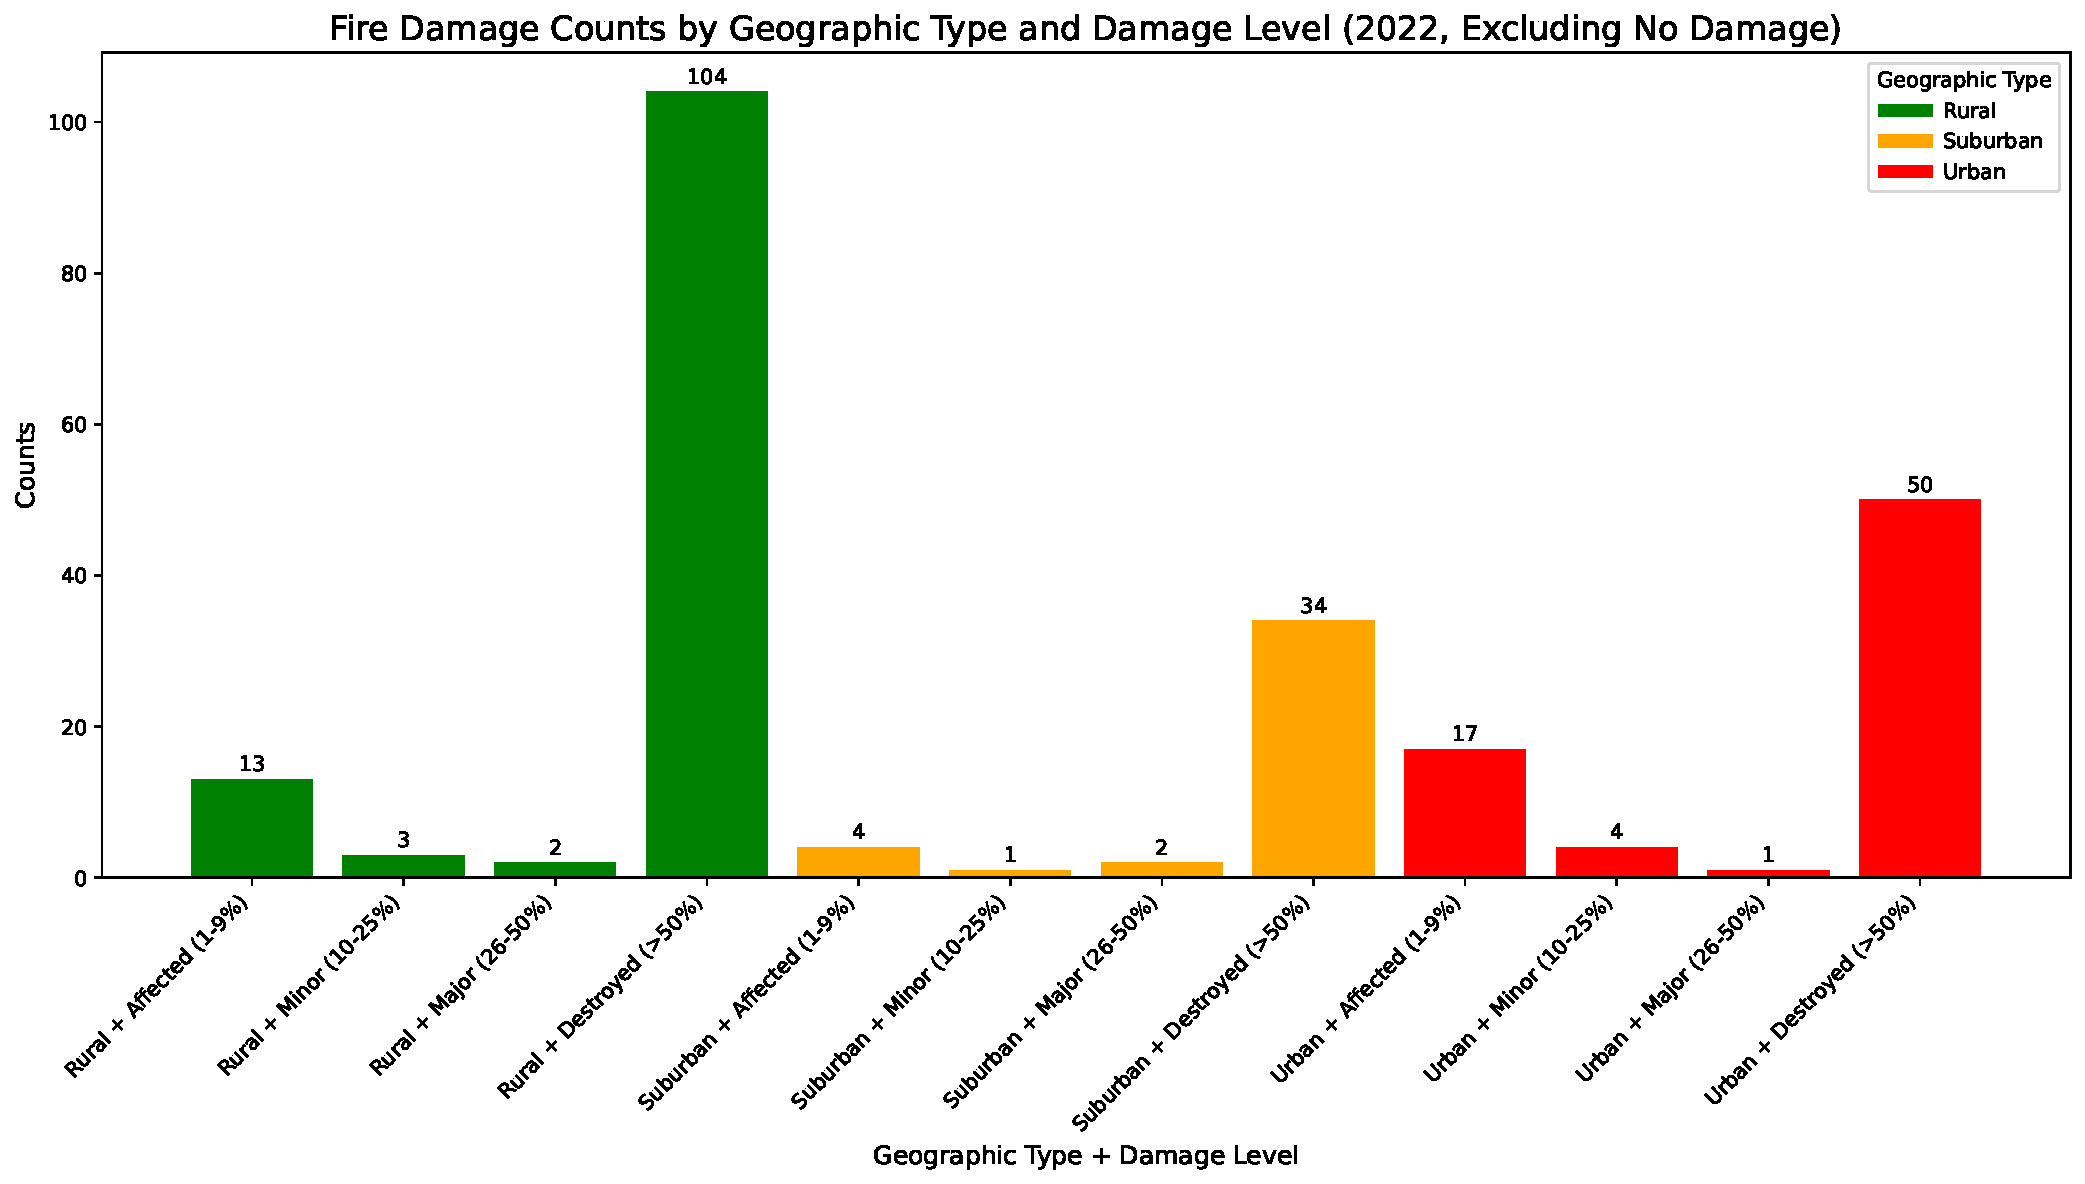
\includegraphics{Final Code_files/figure-pdf/cell-16-output-1.pdf}

\section{plot of 2023 (done by Regina
Hou)}\label{plot-of-2023-done-by-regina-hou}

\begin{Shaded}
\begin{Highlighting}[]
\CommentTok{\# Filter for 2023 data only after merging}
\NormalTok{merged\_data[}\StringTok{"Year"}\NormalTok{] }\OperatorTok{=}\NormalTok{ pd.to\_datetime(merged\_data[}\StringTok{"Incident Start Date"}\NormalTok{], errors}\OperatorTok{=}\StringTok{"coerce"}\NormalTok{).dt.year}
\NormalTok{merged\_data\_2023 }\OperatorTok{=}\NormalTok{ merged\_data[merged\_data[}\StringTok{"Year"}\NormalTok{] }\OperatorTok{==} \DecValTok{2023}\NormalTok{]}
\end{Highlighting}
\end{Shaded}

\begin{verbatim}
/var/folders/r4/x5b99tvj66zcn_88m3jn4r6w0000gn/T/ipykernel_22943/897568859.py:2: UserWarning:

Could not infer format, so each element will be parsed individually, falling back to `dateutil`. To ensure parsing is consistent and as-expected, please specify a format.
\end{verbatim}

\section{plot for 2020-2023 (done by Regina
Hou)}\label{plot-for-2020-2023-done-by-regina-hou}

\begin{Shaded}
\begin{Highlighting}[]
\NormalTok{merged\_data[}\StringTok{"Year"}\NormalTok{] }\OperatorTok{=}\NormalTok{ pd.to\_datetime(merged\_data[}\StringTok{"Incident Start Date"}\NormalTok{], errors}\OperatorTok{=}\StringTok{"coerce"}\NormalTok{).dt.year}
\NormalTok{merged\_data\_total }\OperatorTok{=}\NormalTok{ merged\_data[(merged\_data[}\StringTok{"Year"}\NormalTok{] }\OperatorTok{\textgreater{}=} \DecValTok{2020}\NormalTok{) }\OperatorTok{\&}\NormalTok{ (merged\_data[}\StringTok{"Year"}\NormalTok{] }\OperatorTok{\textless{}=} \DecValTok{2023}\NormalTok{)]}

\CommentTok{\# Group data by geographic type and damage level for 2020{-}2023 combined and sum counts}
\NormalTok{damage\_counts\_total }\OperatorTok{=}\NormalTok{ (}
\NormalTok{    merged\_data\_total.groupby([}\StringTok{"geographic type"}\NormalTok{, }\StringTok{"* Damage"}\NormalTok{])}
\NormalTok{    .size()}
\NormalTok{    .reset\_index(name}\OperatorTok{=}\StringTok{"Count"}\NormalTok{)}
\NormalTok{)}
\end{Highlighting}
\end{Shaded}

\begin{verbatim}
/var/folders/r4/x5b99tvj66zcn_88m3jn4r6w0000gn/T/ipykernel_22943/857330891.py:1: UserWarning:

Could not infer format, so each element will be parsed individually, falling back to `dateutil`. To ensure parsing is consistent and as-expected, please specify a format.
\end{verbatim}

\begin{Shaded}
\begin{Highlighting}[]
\CommentTok{\# Filter for 2020{-}2023 data and exclude "No Damage"}
\NormalTok{merged\_data\_total }\OperatorTok{=}\NormalTok{ merged\_data[}
\NormalTok{    (merged\_data[}\StringTok{"Year"}\NormalTok{] }\OperatorTok{\textgreater{}=} \DecValTok{2020}\NormalTok{) }\OperatorTok{\&} 
\NormalTok{    (merged\_data[}\StringTok{"Year"}\NormalTok{] }\OperatorTok{\textless{}=} \DecValTok{2023}\NormalTok{) }\OperatorTok{\&}
\NormalTok{    (merged\_data[}\StringTok{"* Damage"}\NormalTok{] }\OperatorTok{!=} \StringTok{"No Damage"}\NormalTok{)}
\NormalTok{]}

\CommentTok{\# Group data by geographic type and damage level, and count occurrences}
\NormalTok{damage\_counts\_total }\OperatorTok{=}\NormalTok{ (}
\NormalTok{    merged\_data\_total.groupby([}\StringTok{"geographic type"}\NormalTok{, }\StringTok{"* Damage"}\NormalTok{])}
\NormalTok{    .size()}
\NormalTok{    .reset\_index(name}\OperatorTok{=}\StringTok{"Count"}\NormalTok{)}
\NormalTok{)}

\CommentTok{\# Define the order of damage levels}
\NormalTok{damage\_order }\OperatorTok{=}\NormalTok{ [}
    \StringTok{"Affected (1{-}9\%)"}\NormalTok{, }
    \StringTok{"Minor (10{-}25\%)"}\NormalTok{, }
    \StringTok{"Major (26{-}50\%)"}\NormalTok{, }
    \StringTok{"Destroyed (\textgreater{}50\%)"}
\NormalTok{]}

\CommentTok{\# Update damage levels for sorting and visualization}
\NormalTok{damage\_counts\_total[}\StringTok{"* Damage"}\NormalTok{] }\OperatorTok{=}\NormalTok{ pd.Categorical(}
\NormalTok{    damage\_counts\_total[}\StringTok{"* Damage"}\NormalTok{], categories}\OperatorTok{=}\NormalTok{damage\_order, ordered}\OperatorTok{=}\VariableTok{True}
\NormalTok{)}

\CommentTok{\# Sort the data by Geographic Type and Damage Level}
\NormalTok{damage\_counts\_total }\OperatorTok{=}\NormalTok{ damage\_counts\_total.sort\_values(by}\OperatorTok{=}\NormalTok{[}\StringTok{"geographic type"}\NormalTok{, }\StringTok{"* Damage"}\NormalTok{])}

\CommentTok{\# Create a new x{-}axis label with rearranged categories}
\NormalTok{damage\_counts\_total[}\StringTok{"Label"}\NormalTok{] }\OperatorTok{=}\NormalTok{ (}
\NormalTok{    damage\_counts\_total[}\StringTok{"geographic type"}\NormalTok{] }\OperatorTok{+} \StringTok{" + "} \OperatorTok{+}\NormalTok{ damage\_counts\_total[}\StringTok{"* Damage"}\NormalTok{].astype(}\BuiltInTok{str}\NormalTok{)}
\NormalTok{)}

\CommentTok{\# Assign colors based on geographic type}
\NormalTok{colors }\OperatorTok{=}\NormalTok{ \{}\StringTok{"Rural"}\NormalTok{: }\StringTok{"green"}\NormalTok{, }\StringTok{"Suburban"}\NormalTok{: }\StringTok{"orange"}\NormalTok{, }\StringTok{"Urban"}\NormalTok{: }\StringTok{"red"}\NormalTok{\}}
\NormalTok{damage\_counts\_total[}\StringTok{"Bar Color"}\NormalTok{] }\OperatorTok{=}\NormalTok{ damage\_counts\_total[}\StringTok{"geographic type"}\NormalTok{].}\BuiltInTok{map}\NormalTok{(colors)}

\CommentTok{\# Plot the bar chart}
\NormalTok{plt.figure(figsize}\OperatorTok{=}\NormalTok{(}\DecValTok{14}\NormalTok{, }\DecValTok{8}\NormalTok{))}
\NormalTok{bars }\OperatorTok{=}\NormalTok{ plt.bar(}
\NormalTok{    damage\_counts\_total[}\StringTok{"Label"}\NormalTok{],}
\NormalTok{    damage\_counts\_total[}\StringTok{"Count"}\NormalTok{],}
\NormalTok{    color}\OperatorTok{=}\NormalTok{damage\_counts\_total[}\StringTok{"Bar Color"}\NormalTok{],}
\NormalTok{)}

\CommentTok{\# Add counts on top of each bar}
\ControlFlowTok{for}\NormalTok{ bar }\KeywordTok{in}\NormalTok{ bars:}
\NormalTok{    yval }\OperatorTok{=}\NormalTok{ bar.get\_height()}
\NormalTok{    plt.text(bar.get\_x() }\OperatorTok{+}\NormalTok{ bar.get\_width() }\OperatorTok{/} \DecValTok{2}\NormalTok{, yval }\OperatorTok{+} \FloatTok{0.5}\NormalTok{, }\BuiltInTok{int}\NormalTok{(yval), ha}\OperatorTok{=}\StringTok{"center"}\NormalTok{, va}\OperatorTok{=}\StringTok{"bottom"}\NormalTok{, fontsize}\OperatorTok{=}\DecValTok{10}\NormalTok{)}

\CommentTok{\# Customize the chart}
\NormalTok{plt.title(}\StringTok{"Fire Damage Counts by Geographic Type and Damage Level (2020{-}2023 Total, Excluding No Damage)"}\NormalTok{, fontsize}\OperatorTok{=}\DecValTok{16}\NormalTok{)}
\NormalTok{plt.xlabel(}\StringTok{"Geographic Type + Damage Level"}\NormalTok{, fontsize}\OperatorTok{=}\DecValTok{12}\NormalTok{)}
\NormalTok{plt.ylabel(}\StringTok{"Counts"}\NormalTok{, fontsize}\OperatorTok{=}\DecValTok{12}\NormalTok{)}
\NormalTok{plt.xticks(rotation}\OperatorTok{=}\DecValTok{45}\NormalTok{, ha}\OperatorTok{=}\StringTok{"right"}\NormalTok{, fontsize}\OperatorTok{=}\DecValTok{10}\NormalTok{)}

\CommentTok{\# Add a legend for the bar colors}
\ImportTok{from}\NormalTok{ matplotlib.lines }\ImportTok{import}\NormalTok{ Line2D}

\NormalTok{legend\_elements }\OperatorTok{=}\NormalTok{ [}
\NormalTok{    Line2D([}\DecValTok{0}\NormalTok{], [}\DecValTok{0}\NormalTok{], color}\OperatorTok{=}\StringTok{"green"}\NormalTok{, lw}\OperatorTok{=}\DecValTok{6}\NormalTok{, label}\OperatorTok{=}\StringTok{"Rural"}\NormalTok{),}
\NormalTok{    Line2D([}\DecValTok{0}\NormalTok{], [}\DecValTok{0}\NormalTok{], color}\OperatorTok{=}\StringTok{"orange"}\NormalTok{, lw}\OperatorTok{=}\DecValTok{6}\NormalTok{, label}\OperatorTok{=}\StringTok{"Suburban"}\NormalTok{),}
\NormalTok{    Line2D([}\DecValTok{0}\NormalTok{], [}\DecValTok{0}\NormalTok{], color}\OperatorTok{=}\StringTok{"red"}\NormalTok{, lw}\OperatorTok{=}\DecValTok{6}\NormalTok{, label}\OperatorTok{=}\StringTok{"Urban"}\NormalTok{),}
\NormalTok{]}

\NormalTok{plt.legend(handles}\OperatorTok{=}\NormalTok{legend\_elements, title}\OperatorTok{=}\StringTok{"Geographic Type"}\NormalTok{, loc}\OperatorTok{=}\StringTok{"upper right"}\NormalTok{, fontsize}\OperatorTok{=}\DecValTok{10}\NormalTok{)}

\NormalTok{plt.tight\_layout()}

\CommentTok{\# Show the plot}
\NormalTok{plt.show()}
\end{Highlighting}
\end{Shaded}

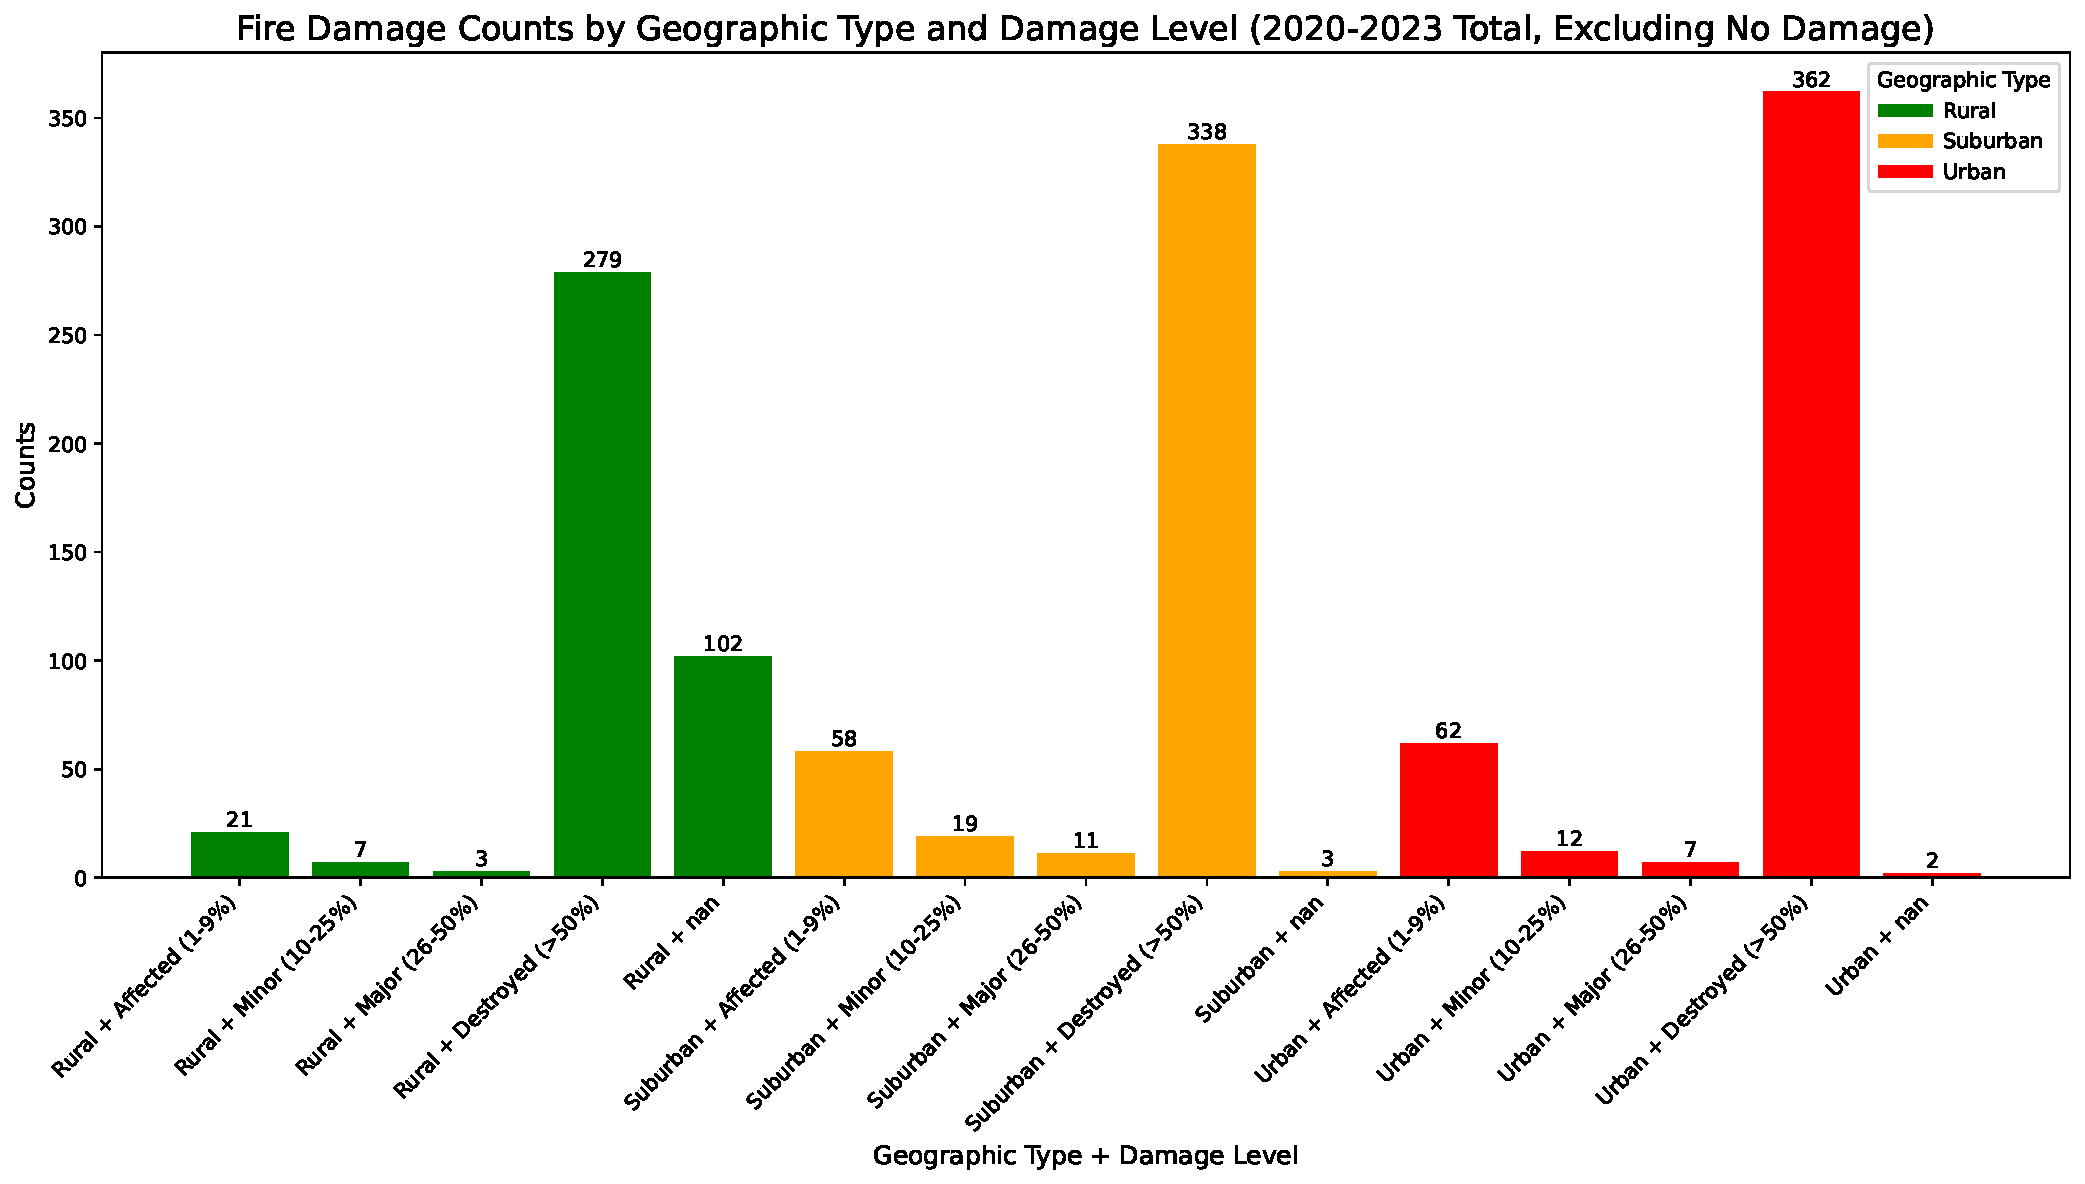
\includegraphics{Final Code_files/figure-pdf/cell-19-output-1.pdf}




\end{document}
